%*****************************************
\chapter{Hand-held object recognition: SHORT dataset, benchmark and the problem of assistive recognition}\label{ch:chapterSHORT}
%*****************************************
%\setcounter{figure}{10}
% \NoCaseChange{Homo Sapiens}


\section{Introduction}
\label{sec:intro}

The ubiquity of smartphones with high quality cameras and fast network connections will spawn many new applications. One of these is visual object recognition, an emerging smartphone feature which could play roles in high-street shopping, price comparisons and similar uses. There are also potential roles for such technology in assistive applications, such as for people who have visual impairment. We introduce the Small Hand-held Object Recognition Test (SHORT), a new dataset that aims to benchmark the performance of algorithms for recognising hand-held objects from either snapshots or videos acquired using hand-held or wearable cameras. We show that SHORT provides a set of images and ground truth that help assess the many factors that affect recognition performance. SHORT is designed to be focused on the assistive systems context, though it can provide useful information on more general aspects of recognition performance for hand-held objects. We describe the present state of the dataset, comprised of a small set of high quality training images and a large set of nearly 135,000 smartphone-captured test images of 100 grocery products. In this version, SHORT addresses another context not covered by traditional datasets, in which high quality catalogue images are being compared with variable quality user-captured images; this makes the matching more challenging in SHORT than other datasets. Images of similar quality are often not present in ``database'' and ``query'' datasets, a situation being increasingly encountered in commercial applications. Finally, we compare the results of popular object recognition algorithms of different levels of complexity when tested against SHORT and discuss the research challenges arising from the particularities of visual object recognition from objects that are being held by users.


There are several motivations for the SHORT dataset; one lies in the emerging application of assistive systems which can help people with visual impairment to obtain information about objects in real-world settings. A common scenario is holding objects whilst either shopping or using items in the house. The familiar platform of camera-equipped smartphones makes image-based query a natural choice for this context. Connected, wearable cameras are, of course, another option.

Image recognition in this context presents very particular challenges, as the variability of viewing conditions (lighting, point of view, etc.) is large. Using Internet-trawled images against which to perform the query is one approach, but it can be expensive if one requires a large number of server-side object-camera poses to guarantee a good quality match. Barcodes are not always easily located by users, and may also be vendor-specific. 

%Therefore the SHORT database aims to incorporate some or all the different conditions that might occur in a real-life shopping scenario and make it difficult. 

The purpose of the SHORT dataset is to provide a useful test of retrieval and object recognition quality when compared against curated databases of high-quality images, which are increasingly being used in search ``Apps'' targeted to particular vertical product markets. 

%In this context, it also allows us to ask the question: how many database shots must be taken for accurate recognition, and how many database shots, covering different poses, are needed to guarantee a certain maximum error rate during a query?


The number of catalogue items -- distinct products, or objects -- in SHORT is currently 100, but the plan is to expand it over time. To some extent, we compensate for this by having a large number of query images -- a total of 134,524 -- taken by as many as 30 mobile phones and including acquisitions from both blindfolded and sighted users. The number and nature of the queries allow SHORT to be used to design and test recognition systems that must place a guarantee on being able to return a correct match. For example, a query image might have to be rejected as being of too low quality to provide a definitive match, either because of visual ambiguity or poor image quality. This is very important in the assistive device context, where rejection of poor quality or ambiguous images would be preferred over simply finding the closest match, which could be catastrophic.

Although our long-term focus is the use of computer vision for assistive devices and systems, SHORT also represents an updated and practical dataset for studying object recognition and retrieval in the challenging scenarios of hand-held objects and mobile or wearable cameras. In this chapter, in addition to introducing SHORT, we provide baseline performance measurements on the current dataset using several object recognition algorithms with different degrees of recognition complexity.

In Section~\ref{sec:related-work} we review the computer vision datasets related with object recognition and argument the need for SHORT on the basis of an increasingly mobile and inclusive world. In Section~\ref{sec:short} we describe the experimental set-up for image acquisition and the particularities of the different datasets that comprise SHORT. Section~\ref{sec:benchmarks} describes the benchmarking of the dataset and its results, illustrating the advantages and disadvantages of the set. These will be discussed in Section~\ref{sec:conclusions}, where we will point out the future work.

\begin{figure}[h!]
\centering
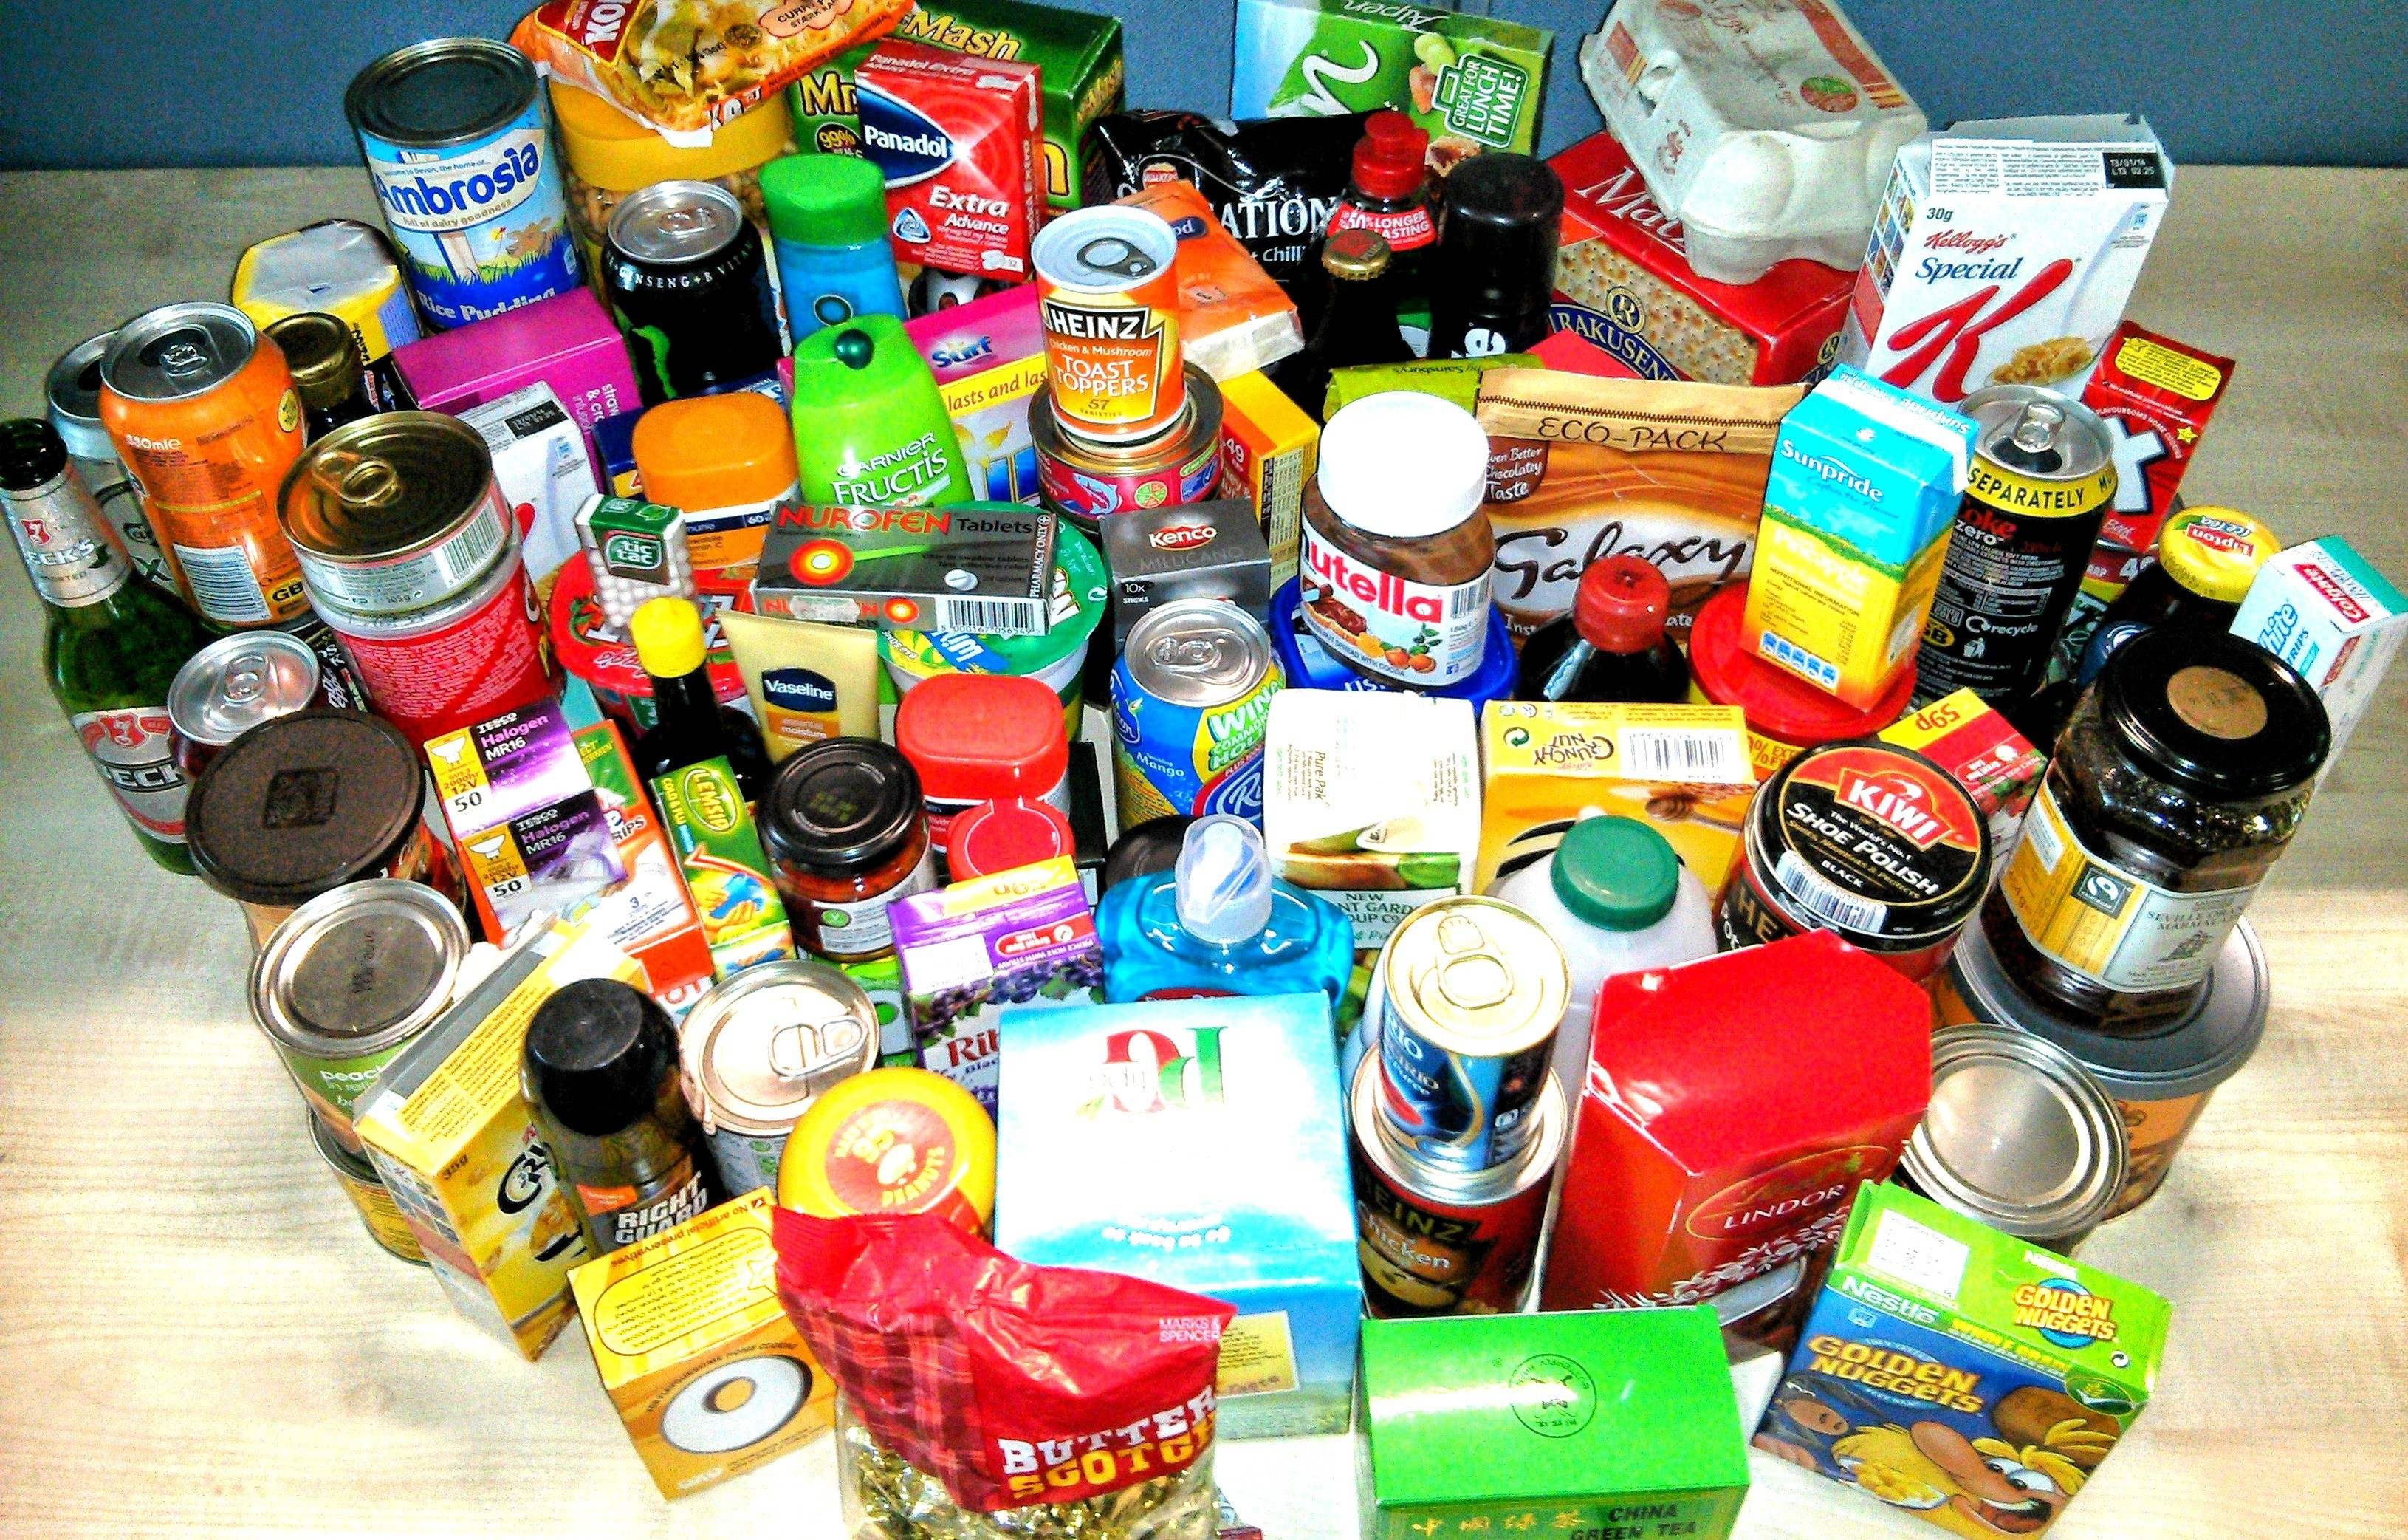
\includegraphics[width=\textwidth]{./gfx/Chapter03/SHORT_family_photo.jpg}
\caption{All the grocery products that compose the SHORT dataset in its final set of 100 categories.}
\label{fig:short-100-all}
\end{figure}


\begin{figure}
\centering
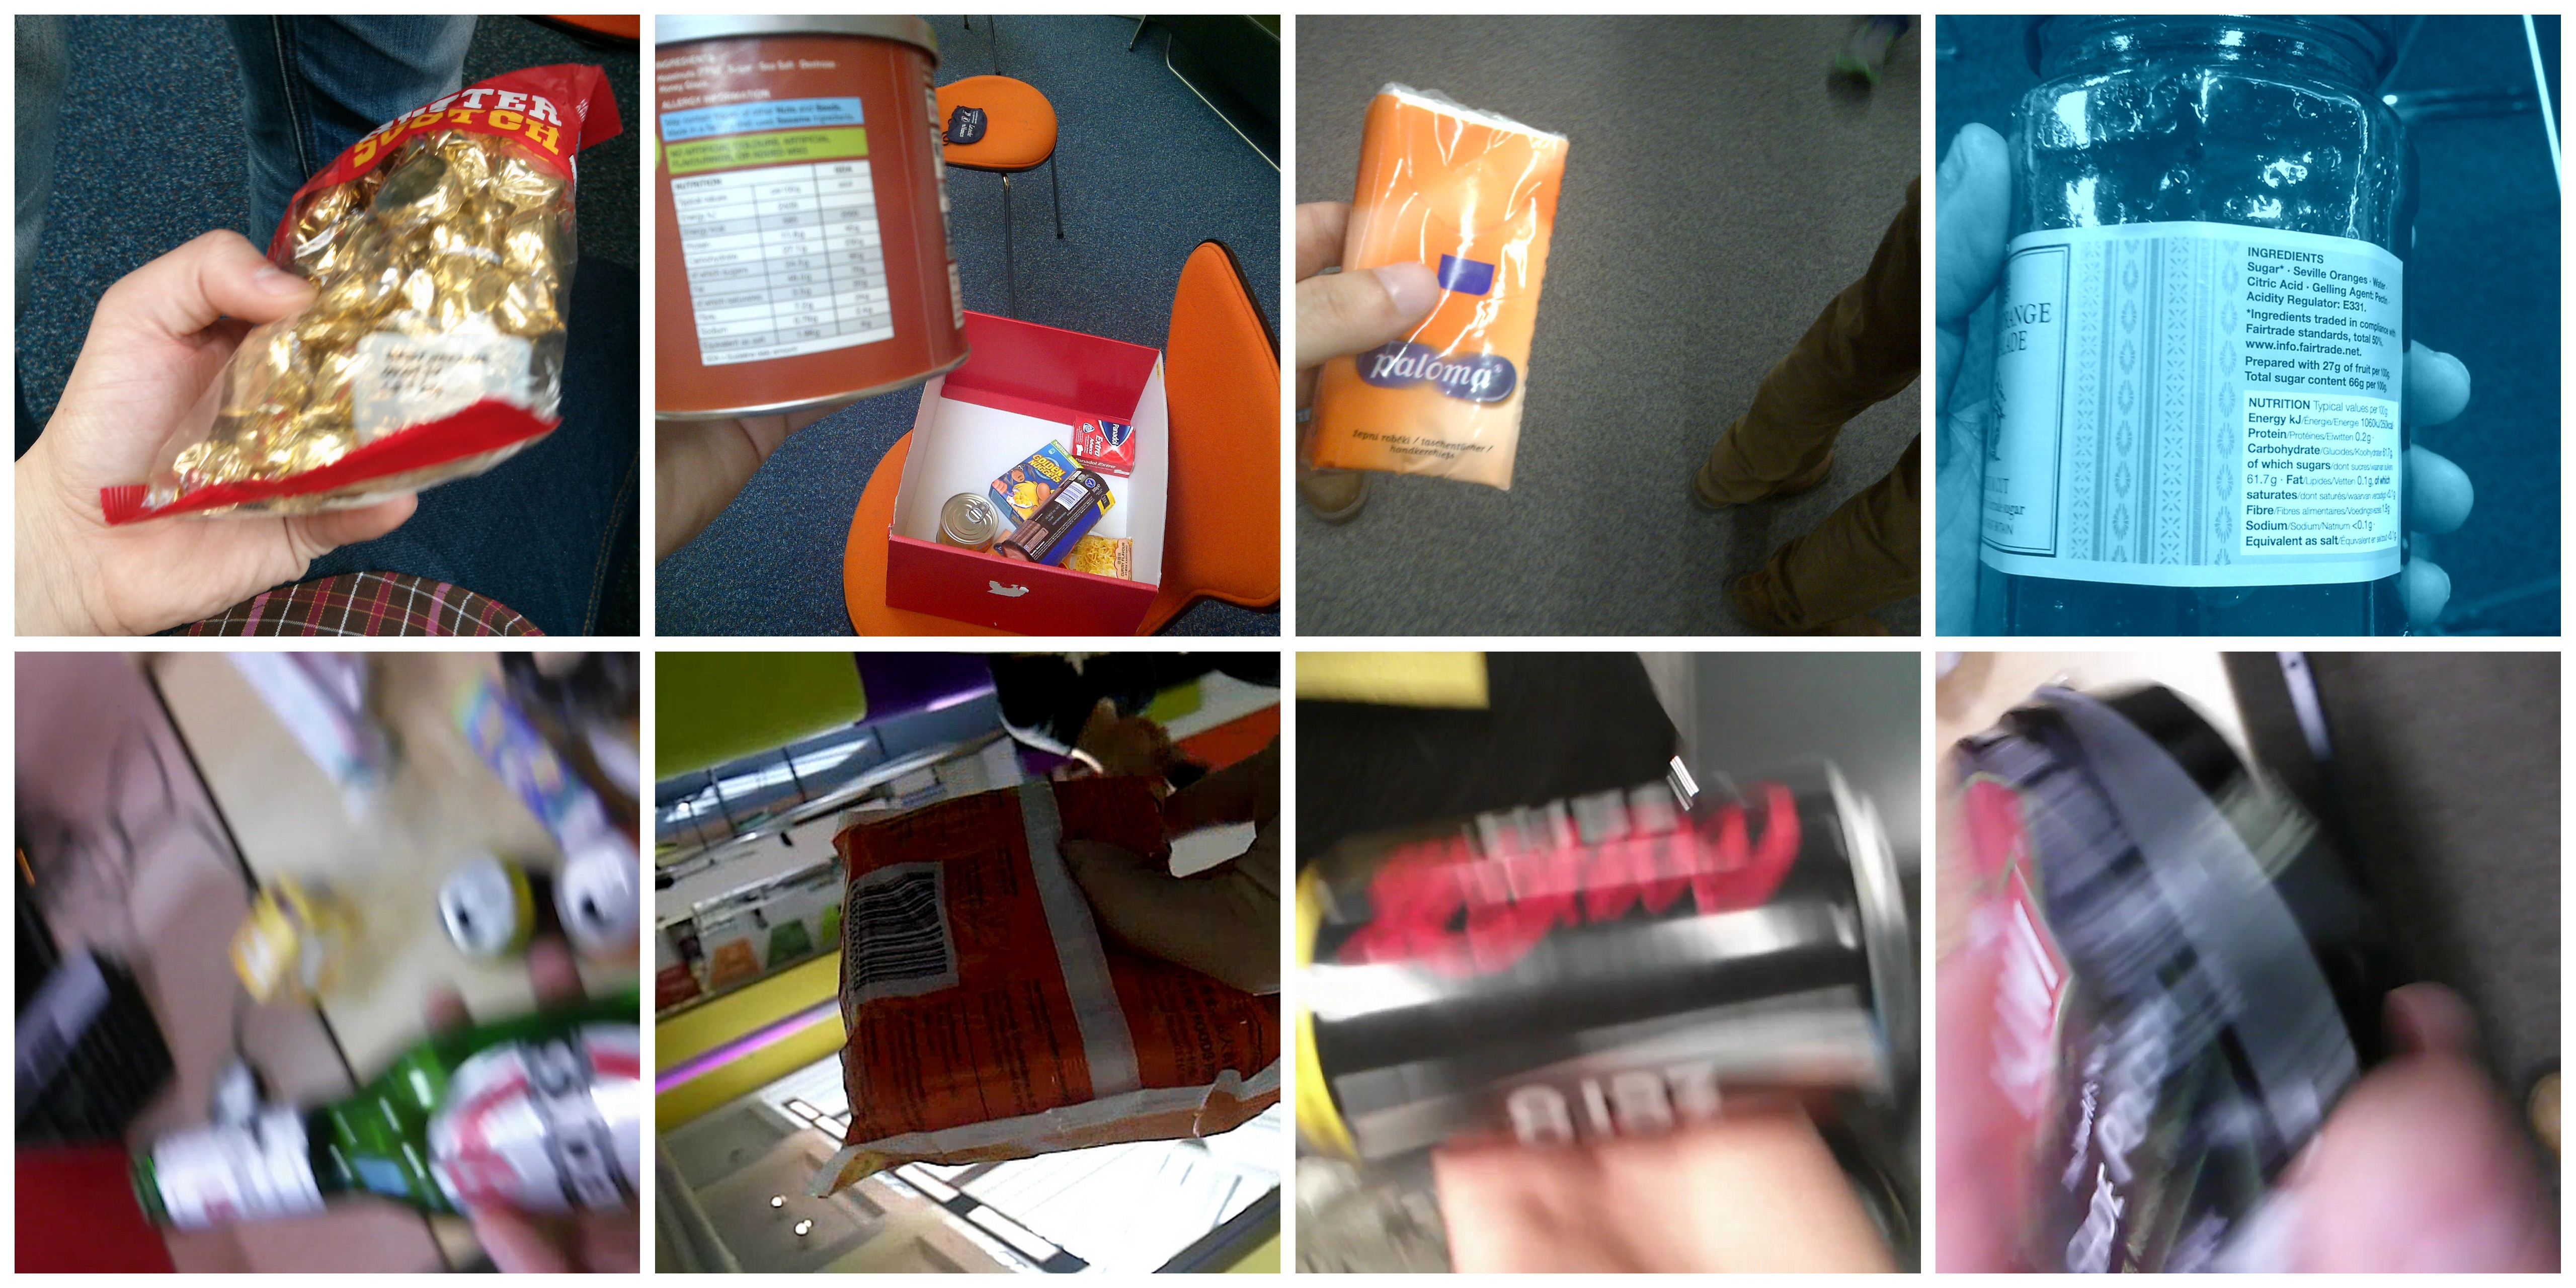
\includegraphics[width=.75\linewidth]{./gfx/Chapter03/icip-test-imgs2.jpg}\label{fig:testSetCollage}
\caption{Sample test images. \textbf{Top row}: still-images; \textbf{bottom row}: video frames. Note: the images were cropped to fit the collage, they actually have different resolutions. This query selection contains samples from all the test datasets (see Table~\ref{table:testData}.)}
\label{fig:short-30}
\end{figure}

%------------------------------------------------------------------------
\section{SHORT and related datasets} \label{sec:related-work}

COIL-100~\cite{Nene1996a} and SOIL-47~\cite{Koubaroulis2002} laid the foundations for the provision of large-databases of objects but their formats, image sizes and depth are now slightly dated.

A related database of house-hold products is the Grozi-120 dataset \cite{Merler2007}. It contains 120 categories of groceries and is divided into ``model'' and ``query'' sets. For every product, the models were downloaded from the Internet while the queries consisted of cropped video frames from recordings of supermarket shelves. SHORT provides a curated database of models to train object recognition algorithms taking also into account the assistive usage context, where the queries are highly variable. Grozi-120, however, lacks the variability and background clutter that would occur in real world scenarios, and the training images only have a limited number of views per product, usually just the frontal one showing the brand. SHORT expands the number of views to 36, with 12 different levels of rotation and 3 elevations.  The multiple views allow us to determine the importance of viewpoint in being able to guarantee a definitive match. 

Caltech-101 and 256 \cite{Feifei2007,Griffin2007}, together with PASCAL VOC~\cite{Everingham2009} have been widely used to train and benchmark object recognition and detection algorithms. Caltech's dataset increased the depth of previous datasets, achieving a minimum of 80 images per category to favour the variability in training and test database size. However, neither dataset is recommended for localisation tests as the images contain ``photographer's bias'' in which the objects are usually placed near the center of the image. Nevertheless, the challenging nature of the PASCAL datasets, and the well-defined evaluation protocol, has led to it being a widely-cited benchmark for object recognition algorithms over recent years. However, only 2 out of 20 categories have a depth larger than 1,000 images per category, while in SHORT the minimum number of images per category is 3,507, outnumbering the latest PASCAL and both Caltech datasets.
 
ImageNet~\cite{Deng2009} was publicly released in 2010 to increase the number of categories up to the level of human recognition, which is estimated to be in the range of the tens of thousands~\cite{Biederman1987}. ImageNet focuses on object categorisation ``at near human scale'' and therefore provides 1.2 million images of a broad range of objects belonging to 1,000 categories~\cite{Feifei2007}. This remarkable dataset depth, however, presents certain disadvantages when the scope of the application is more specific, as it is in the context of shopping or assistive systems. The 100 products from SHORT, and the ones that will be obtained for subsequent expansions, are widely available. However, only 6 out of the 100 can be found in ImageNet: Coca-Cola, orange Fanta, semi-skimmed milk, orange marmalade, deodorant and OXO chicken cubes. From these some presented ambiguities: the category milk contained 231 images; some represented milk bottles valid for a shopping context, but some of them depicted a glass or jug of milk, milk crates in a factory, or other packages of milk. ImageNet cannot be used to train a system that guarantees a minimum scalability in a shopping context. Another criticism lies in the fact that some specific items are hard to index. In ImageNet, for instance, the orange Fanta is under drinks $\rightarrow$ soft drinks $\rightarrow$ orange synset. This makes it difficult to use ImageNet as a benchmark dataset for such a specific application.


While some of the datasets mentioned above, like Pascal and ImageNet, offer a high degree of variability, SHORT has been designed to target the specific need of a dataset to develop object recognition systems in the context of hand-held queries, particularly for use in assistive devices.

Another important limitation of existing datasets is that they use large amounts of training data containing unsystematic views of an object to train classifiers; this introduces bias and can lead to ``solving'' the dataset. SHORT, however, offers a training set of model images which systematically cover variations in an object's viewing angle. This allows to study how recognition of queries taken non-systematically is affected by the variability in viewpoints in the training data.

Test images from many datasets lack the variability in views or introduce the photographer's bias. On the other hand, the image queries in SHORT have been captured by multiple users with a variety of the latest smartphone cameras covering a wide range of viewing angles and containing images at current typical resolutions. This context is not covered by traditional datasets, in which high quality catalogue images are being compared with variable quality user-captured images; this makes the matching more challenging in SHORT than other datasets. Images of similar quality are often not present in both ``database'' and ``query'' datasets, a situation being increasingly encountered in commercial applications.

As an additional feature SHORT also contains test images acquired by blindfolded users and therefore mimics scenarios involving visually impaired users. 

We have not performed experiduments with visually impaired users to date, because for each potential assistive application (e.g. recognition, navigation), our protocols require that we demonstrate performance in sighted, then blindfolded users first, before conducting trials with visually-impaired volunteers. 

%%-------------------------------------------------------------------------
\section{SHORT technical details} \label{sec:short}

\subsection{Overview}

SHORT is comprised of separate datasets for training and testing. Currently, the training dataset consists of high resolution acquisitions of 100 grocery items acquired in a very controlled set-up (see Figure~\ref{fig:acqsetup}), with 36 images of the same object from different angles and views. For testing, we provide a set of query images of a subset of 30 grocery items acquired with 30 different smartphones. Lighting, pose, sensors and optics were quite varied. This represents a more realistic view of hand-held object queries from hand-held devices. The SHORT dataset contains an average of more than 4,200 queries per product, allowing a realistic study of factors that affect recognition quality. In addition, video sequences of hand-held objects contain blur and different background clutter, as the volunteers moved while capturing sequences, relevant to a use case that might be considered as streamed object recognition. 



In addition to the images, we provide ground truth annotations for all the data in terms of its object class label. We also include binary masks of the objects from the training dataset, indicating the bounding box around each item.

SHORT is openly available and it can be downloaded from \cite{Rivera-Rubio}. The website  \url{http://short.bicv.org} includes contact information where database users and SHORT curators can exchange impression for future releases. The website provides access to the data as a single download or through a web file sharing service based on the open-source Owncloud that allows browsing. This contains access to the two releases of the dataset: SHORT-30 and SHORT-100. The original acquisition took place during the summer of 2013. The expansion of SHORT took place in June 2014 after taking into account feedback from the community on the usability of SHORT. The release of the dataset also includes code and evaluation data.

\subsection{Image acquisition protocol}

\subsubsection{Training images}

The database of models was acquired with a Nikon D7000 SLR camera using a 18-105 mm lens connected to a laptop and using the Nikon \textit{live capture} software. The 16.2 megapixel captures in \textit{raw} format were kept, but a JPEG copy of each image was also generated with a resolution of 4928$\times$3264 pixels. A 986$\times$653 resized copy of the high resolution images is also made available

A total of 36 views were acquired per category. The views used in the product models contain shots at three elevations (17, 47 and 68 cm, at a distance of 1m) above the object base. 12 degrees of rotation were used per elevation. A professional ``chroma key'' set-up was used. Both the background and a turntable containing the object were covered with a uniform chroma key backdrop, a ``chroma blue'' and ``chroma green'' cloth depending on the main color of the product being shot. Two halogen 125 W (equivalent to 625 W) 5500 K lamps were used to illuminate the background whilst the object was illuminated with a 40 $\times$ 40 cm 5400 K LED panel. The set-up is shown in Figure \ref{fig:acqsetup}.


\begin{figure}
\centering
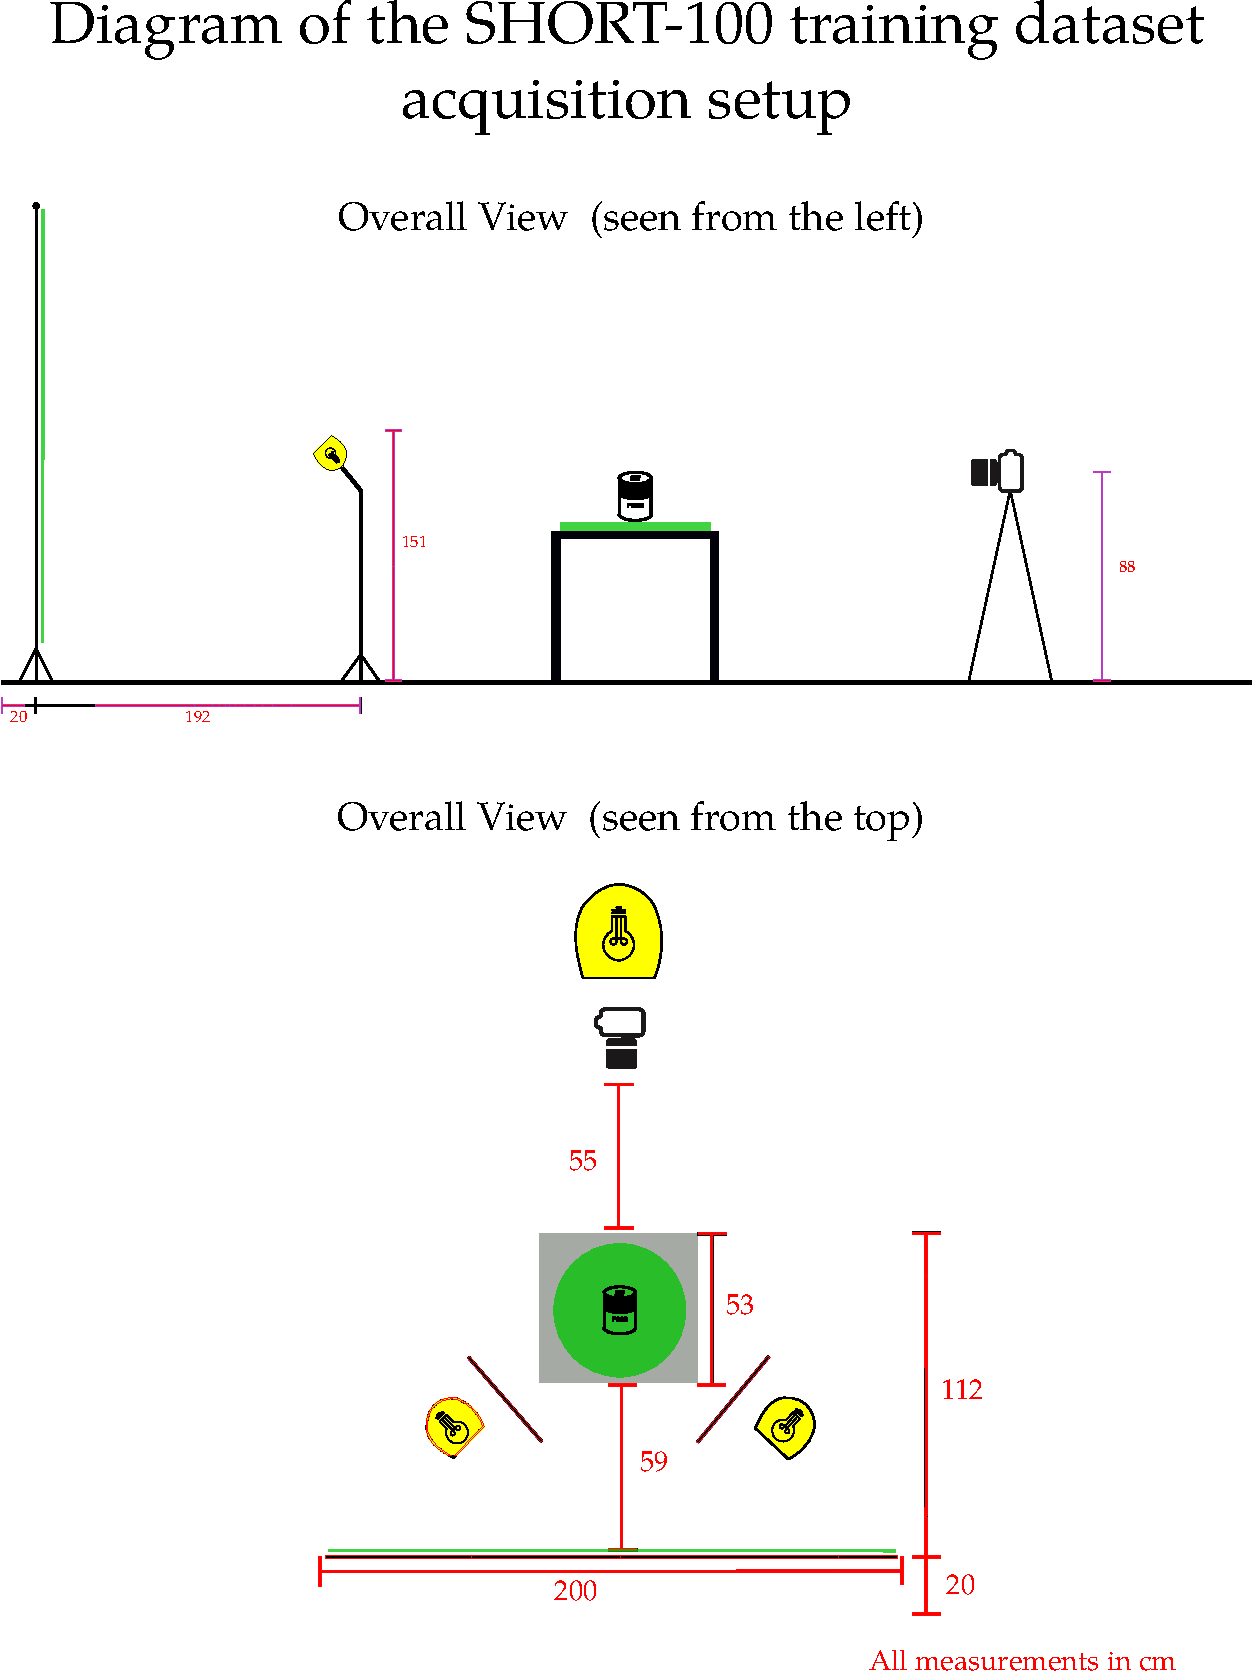
\includegraphics[width=\linewidth]{gfx/Chapter03/acquisition_diagram.pdf}
\caption{SHORT training set acquisition set-up}
\label{fig:acqsetup}
\end{figure}

As described above, the acquisition of the training images was divided in two phases. In the first, model images of 30 products (the same set as the test set) were acquired. After receiving feedback from the community, we planned a second acquisition phase to expand the number of categories to 100 and allow for the generalisation of the algorithms tested with the dataset. The products of SHORT-30 are shown in the collage in Figure~\ref{fig:collage-all}.

\begin{figure}[]
\centering
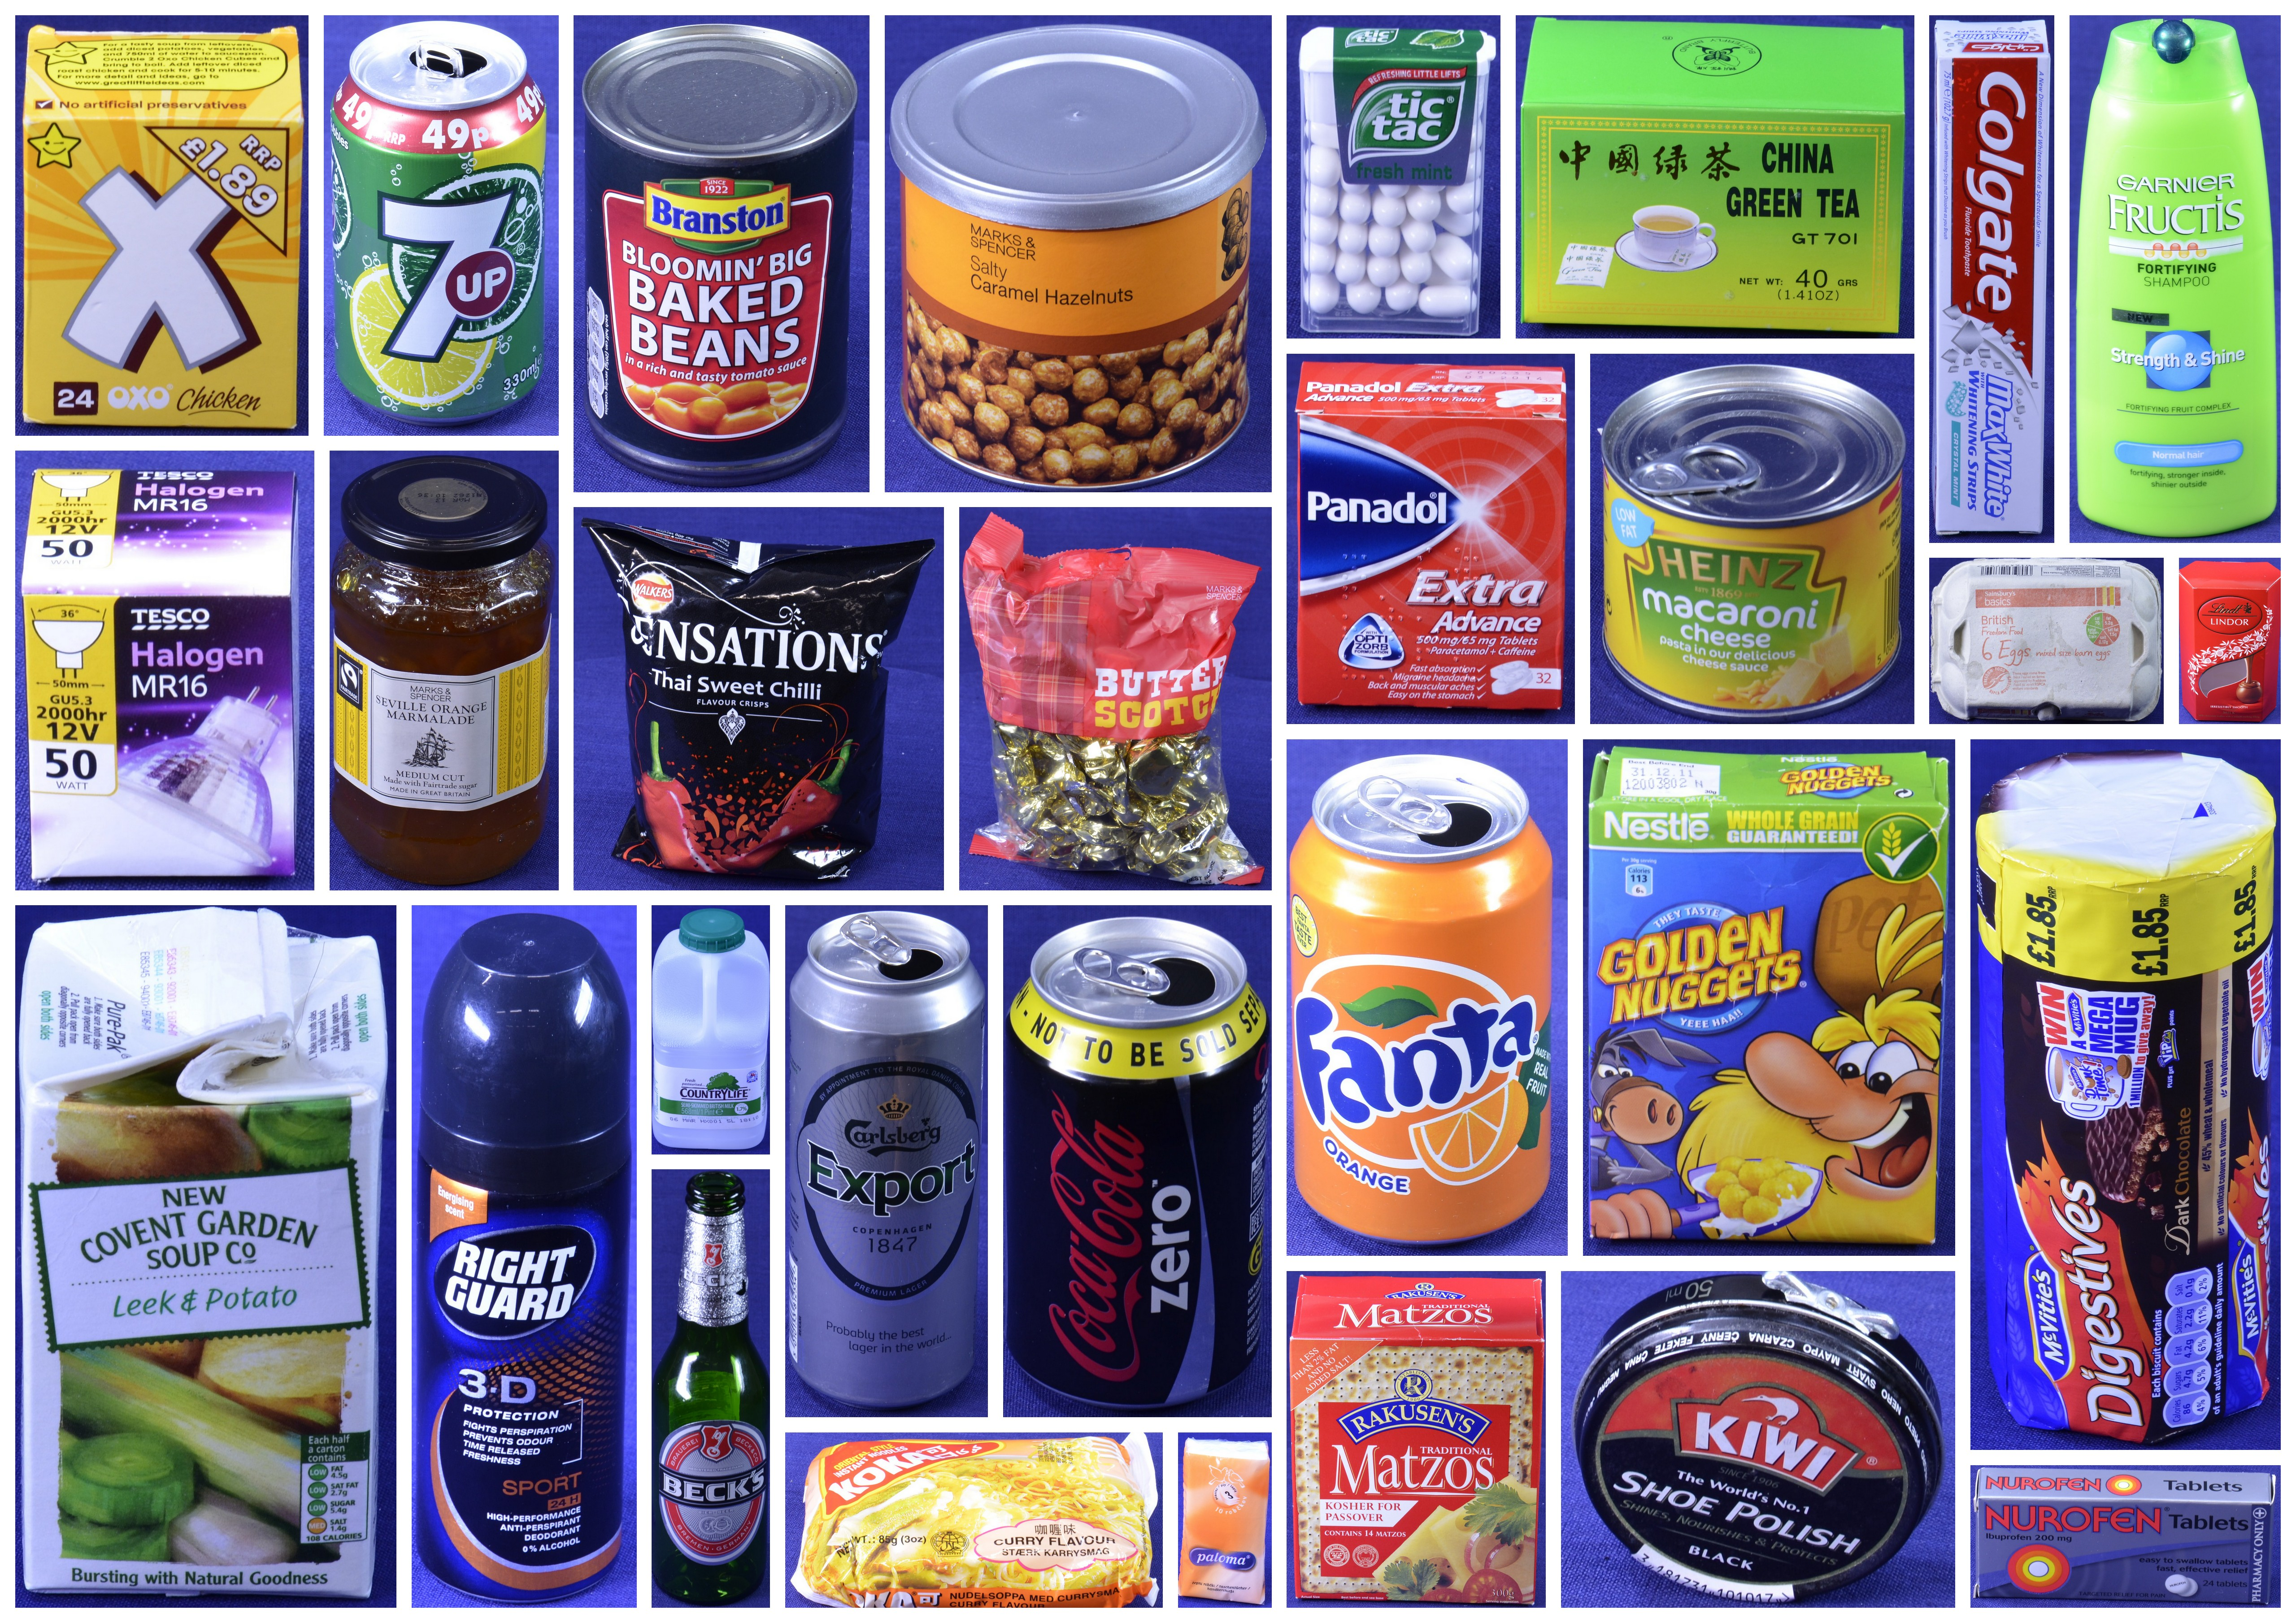
\includegraphics[width=\textwidth]{./gfx/Chapter03/icip-all-products.jpg}
\caption{Collage representing the grocery products in the SHORT-30 dataset. This is a selection of items to include cans (shiny), boxes, uneven surfaces, similar shapes, semi-transparent or deformable packaging. These are popular products that are widely available for easy reproducibility and contain snacks, toiletries, medicines, drinks, canned food, dairy products, etc. Figure~\ref{fig:short-100-all} shows all the products in the final SHORT-100 release.}
\label{fig:collage-all}
\end{figure}


The process described above produces high-quality database (training) images; however we took no such precautions with the query (test) images. The difference in capture quality makes SHORT very relevant to the usage case that we have outlined, in which high-quality product images are used to provide a controlled database of items.  We see this factor as very important in order to quarantee the quality of information.  Such multi-view images are routinely acquired for product catalogues, marketing brochures, and websites, forming a standard part of the product manufacturing processes.

\subsubsection{Test images}

Two experimental sessions were conducted. Volunteers were asked to take a minimum of five shots of every product and a five second video. No other instructions were given on how to acquire the images. During the second acquisition experiment, the images were taken with blindfolded users, reducing the alignment bias that a sighted user might have; we used this as a proxy for the assistive device context.  Visually-impaired users will also be recruited once the quality of search can be demonstrated as being sufficient for real-world use.

\begin{table}
\begin{center}
\begin{tabularx}{\textwidth}{XXXXX} \toprule
 \tableheadline{Dataset} & \tableheadline{Total Images} & \multicolumn{3}{c}{\spacedlowsmallcaps{Images Per Category}}\\
& & \spacedlowsmallcaps{Min} & \spacedlowsmallcaps{Max} & \spacedlowsmallcaps{Mean} \\
\midrule
ST-SG & 2,797 & 75 & 115 & 93.23\\
\midrule
VF-SG &  91,293 &  2,115 & 4,033 & 3,043.10 \\
\midrule
ST-BF & 1,225 & 32 & 57 & 40.83\\
\midrule
VF-BF &  39,209 &  832 & 1,884 & 1,306.97 \\
\midrule
All &  134,524 &  3,054 & 6,089 & 4,213.9 \\
\bottomrule
\end{tabularx}
\end{center}
\caption{Summary of SHORT test datasets. Still images (ST) and videoframes (VF) acquired by sighted users (SG) or blindfolded (BF).}
\label{table:testData}
\end{table}

A total of 30 different camera-equipped smartphones was used, with resolutions ranging from 320$\times$240 to 3264$\times$2448 pixels. The variability of camera characteristics, parameters and capture conditions is enormous and a very distinctive feature of this dataset. The collage shown in Fig. \ref{fig:testSetCollage} contains a small sample of the  variability present in the test dataset. As can be appreciated, images contain different views, levels of sharpness, background clutter, occlusion, illumination, and specular reflection. These realistic features of the queries, together with the availability of sighted and blindfolded sets, help in identifying certain characteristics required for database quality and coverage in order to meet the assistive and hand-held usage contexts. 
%For example, for a partially sighted user, or one who is not certain where the front of the object is, the database will need to contain more than one view. How many views is, of course, dependent on the object; and determining the necessary number of views is a common requirement that one encounters when building commercial or public-service search services within finite budgets and compute resources.


%%------------------------------------------------------------------------
\section{Benchmarks} \label{sec:benchmarks}


%\subsection{Methods}


%%%%%%%%%%%%%%%%%%%% SIFT PAIRWISE
\subsection{Classification using SIFT Descriptor Matching}
% Baseline for descriptor matching based methods

Object recognition can use several properties of query and database image appearance, ranging from colour distributions to texture and gradient field fingerprints \eg histograms of gradients (HoG). However, apart from the use of spatial arrangements of putative matches between datasets and images, the discrimination of visual words, or bags of visual words, is unlikely to be able to exceed the discrimination power of the descriptors or fingerprints used.

For this reason, we include an evaluation of the performance of an object recognition algorithm using a variant on pairwise SIFT ~\cite{Lowe2004} descriptor matching for generating scores between a query and each model image in the training dataset. Each match is ranked according to a distance score; the match with the lowest distance score is assigned the highest ranked similarity. A query is then classified into one of the object classes. We now describe the basic matching technique in more detail.

Let us consider $N$ training images $\mathbf{T}^{(n)}, n = 1, 2, ..., N$. A SIFT database was first constructed by computing $I^{(n)}$ descriptor vectors $\mathbf{y}_i^{(n)}, i = 1, 2, ..., I^{(n)}$ using VLFEAT~\cite{Vedaldi2008}. Each descriptor is of dimension $128\times 1$, so is in line with the commonly used configuration, as described by Lowe~\cite{Lowe2004}.

Consider, now, a query image, $\mathbf{Q}$ yielding $J$ SIFT descriptor vectors, $\mathbf{x}_j, j = 1,2,...,J$. The Euclidean distance~\cite{Vedaldi2008} in descriptor space was first computed between query descriptors, $\mathbf{x}_j$, and the training set descriptors, $\mathbf{y}_i^{(n)}$, for each training image, $\mathbf{T}^{(n)}$. Distances were then sorted for each compared descriptor pair.  This was repeated for each image, yielding sets $\mathcal{U}^{(n)}$ consisting of tuples of indices $(p,q)$ such that
\[
\mathcal{U}^{(n)} := \lbrace (p,q): f_\mathcal{U}(\mathbf{x}_q,\mathbf{y}_p^{(n)})=1\rbrace,\,\,\forall n
\]
where $f_{\mathcal{U}}$ is a uniqueness criterion on descriptor distances within each image pair; we used the implementation of VLFEAT~\cite{Vedaldi2008}, based on the approach suggested by Lowe~\cite{Lowe2004} to define the set of matching descriptor pairs between the query image, $\mathbf{Q}$, and each training image, $\mathbf{T}^{(n)}$. $f_{\mathcal{U}}$ is defined so that descriptor pairs which meet the criterion evaluate to 1, and otherwise to 0. 

For {\em each} of the $K^{(n)}$ descriptor pairs $(p,q)$ that pass the uniqueness test $f_{\mathcal{U}}$ for each training image $n$, we can calculate the pairwise distances in descriptor space:
\begin{equation}
d_k^{(n)} =  ||\mathbf{x}_q-\mathbf{y}_p^{(n)}||, \quad k = 1,2,...,K^{(n)}
\label{EucDistance}
\end{equation}
where $K^{(n)} = |\mathcal{U}^{(n)}|$ is the number of descriptor matches after filtering for uniqueness. A scaled average of the distances $d_1^{(n)},d_2^{(n)},...,d_{K^{(n)}}^{(n)}$ is then computed~\cite{Li2009} to give a single estimate $\mu^{(n)}$ of the distance between query image and training image:

\begin{equation}
\mu^{(n)} = \frac{1}{K^{(n)}}\frac{\sum_{k=1}^{K^{(n)}} d_k^{(n)}}{K^{(n)}}
\label{eqScore}
\end{equation}

Smaller $\mu^{(n)}$ for a candidate database image, $\mathbf{T}^{(n)}$, implies a higher similarity and thus a stronger match.
%"This creates a score space"...
A query $\textbf{Q}$ is then classified as belonging to the class $C^{(p)}$ corresponding to the training image $\mathbf{T}^{(p)}$ if

\begin{equation}
p = \underset{n}\argmin\lbrace \mu^{(n)}\rbrace
\end{equation}

\noindent with $C^{(p)} \in \lbrace 1, 2,..., N_P\rbrace $ and where $N_P$ is the number of product classes.

This descriptor-based method is likely to be indicative of the discriminating capacity of individual descriptor types; it is likely that this will have some effect on the ultimate performance of an object recognition technique. However, because it relies on descriptor-by-descriptor comparison, it is not readily scalable to large database sizes. Nevertheless, we keep it as one type of ``gold standard'' method, despite not encoding geometric relationships between keypoints. We compare this with the performance of more scalable techniques in Section~\ref{sec:results}.

%% OLD STUFF

%\begin{equation}
%\begin{array}{cccc}
%q^C \longleftarrow n^C & \text{if} & \frac{S_n}{S_m} < \Theta & \\
%\text{where} & m \neq n & \text{and} & m^C \neq n^C
%\end{array}
%\end{equation}

%The threshold, $\Theta$, was set in order to reject queries having a close match score between two object classes. Different threshold values were evaluated on a subset of 100 randomly chosen queries across 10 trials and it was observed that increasing the threshold increased the true positive rate but also the false positive rate due to the classification being less conservative. A threshold $\Theta$ was set to a value of 0.8 for further analysis as this led to the highest accuracy. This method was previously used by Lowe~\cite{Lowe2004} to discard weak matches but at descriptor level. We show that the same method can be applied at image level which will reject queries with weak matches rather than classifying them as false positives. The classification accuracy however remains low due to the conservative nature of this method but yields a high classification precision, which is imperative in the context of assistive devices. Such methods can pave the way towards applying additional quality tests on queries in order to reject low quality (blurred, overexposed, \etc).
%
%\paragraph{Results} The classifier performance was measured using classification accuracy, precision and recall as suggested by~\cite{Fawcett2006} -- these definitions are not to be confused with the terms used in the object retrieval context. Accuracy was given as the percentage of correct matched (true positives) from all queries; precision and recall were calculated as percentage of true positives from all the predicted positives and percentage of true positives from all the actual positives, respectively.
%


%%%%%%%%%%%%%%%%%%%%% SIFT PAIRWISE End.... 


%%% BOVW STARTS

\subsection{Benchmarking: More Scalable Approaches}
\label{sec:bof}

The challenges posed by this dataset was also assessed using a fairly standard recognition ``pipeline'' to provide category (product ID) ranking. The SIFT descriptor was applied in one of two approaches: dense or sparse. The dense approach employs a grid with either 3 or 8 pixel spacing, and a 16$\times$16 spatial extent for the single-scale approaches. The sparse approach uses keypoint detection with standard SIFT-based scale-selection. The VLFEAT implementation is used for the descriptor-keypoint acquisition. Three different histogram encoding methods were applied: hard assignment \cite{Csurka2004} (using 400 and 4000 visual words), Locality-Constrained Linear coding (LLC) \cite{Wang2010} and Fisher Vector (FV) encoding \cite{Perronnin2010}. We used the set-up of Chatfield et al. for the FV approach as it is known to perform best~\cite{Chatfield2011}.These methods will be described separately below. 

On top of LLC and FV, spatial pyramids pooling was applied, using the approach described in~\cite{Lazebnik2006} and with 3 pyramidal levels (0,1,2). Kernels (as defined in \cite{Vedaldi2010}) were first computed for each pyramidal feature~\cite{VanDeSande2010}. Kernels were then averaged and fed to an SVM to determine the classification accuracy and average precision. The LibSVM implementation~\cite{CC01a} was used to train an SVM for each category. The average precision values that are reported are in direct accordance with the VOC evaluation protocol~\cite{Everingham2009}. 

\paragraph{Hard Assignment} 
In hard assignment, a visual word is mapped to the closest matching descriptor within an image ~\cite{Csurka2004}. The visual words are generated using the $k$-means clustering algorithm to generate codebooks of 500 and 4000 visual words: these sizes allow performance comparisons with techniques reported in the literature. A feature vector was constructed for each image by counting the occurrences of the visual words present in that image. For this case, an SVM with a linear kernel was applied to perform classification. 

\paragraph{Locality-constrained Linear Coding (LLC)} 
In some studies, LLC~\cite{Wang2010} has been found to yield better recognition performance than hard assignment. Each descriptor is then encoded with a weight vector, $\mathbf{w}$, based on the covariance matrix, $\mathbf{C}$, of its distances to the 5 nearest neighbours by solving $(\mathbf{C} + \lambda \mathbb{I}_{5})\mathbf{w} = \mathds{1}_{5\times 1}$ with $\lambda=10^{-6}$ and where $\mathbb{I}_n$ is the $n\times n$ identity matrix and $\mathds{1}_{m\times 1}$ denotes a column vector of $m$ elements containing 1. This method has been shown to work well with linear classifiers, allowing relatively simple implementation.
% Old text
%In some studies, LLC~\cite{Wang2010} has been found to yield better recognition performance than hard assignment. The histogram encoding is performed by finding the 5 nearest descriptors to each visual word, using the same codebooks as described in the paragraph above. The covariance matrix of the 5 nearest neighbours was projected to a unit vector and the maximum response from this vector was used to select each visual word. This method has been shown to work well with linear classifiers, allowing relatively simple implementation.
\paragraph{Fisher Vector Encoding} 
Fisher vectors have been shown to produce state-of-the-art performance in popular classification benchmarking datasets \cite{Chatfield2011}. Recent work~\cite{Perronnin2010} has shown that the classification performance can be boosted even further by using a dense multi-scale approach. Thus, the set-up of Chatfield et al. ~\cite{Chatfield2011} was followed to determine the classification rates by using 4 scales of analysis with two different sampling densities of 3 and 8 pixels. The spatial bin size of the SIFT descriptor was changed to $4,6,8$ and $10$ for each of the 4 scales, respectively. The descriptor dimensionality was reduced to 80 elements by using Principal Components Analysis (PCA) and fitting a Gaussian Mixture Model employing 256 components. The Fisher vector encoding was obtained by finding the closest descriptor for each Gaussian model and aggregating the first and second order statistics. Finally, a Hellinger kernel, known to perform best for this type of encoding, was used to train the SVM classifier.

%%% BOVW ENDS

%------------------------------------------------------------------------

\section{Analysis} \label{sec:analysis}

% Metrics
\subsection{Metrics}
Several metrics exist for evaluating a classifier's performance. For each query, a one-against-all binary classifier leads to four possible outcomes: \emph{true positives (TP)}, \emph{false positives (FP)}, \emph{true negatives (TN)} and \emph{false negatives (FN)}. With these definitions, we can derive common performance metrics in the classification context given $P$ and $N$ the number of positive and negative queries respectively: \textbf{Classification accuracy} can be defined as the fraction of queries correctly classified ($\frac{TP+TN}{P+N}$). \textbf{Precision/Recall} (PR) curves, generated by arranging all the queries in descending order of their classification score~\cite{Everingham2009} (\ie the ranked output or confidence of how strong the prediction is). \textbf{Recall} can then be defined as the proportion of all positive queries with a classification score higher than a threshold. \textbf{Average Precision} (AP): the area under the PR curve. Mean Average Precision (\textbf{mAP}): the mean average precision for a set of queries, and ultimately, the mean AP across classes.

%\begin{itemize}
%\item $\text{Precision} = \frac{TP}{TP+FP}$
%\item $\text{Recall} = \frac{TP}{P}$
%\end{itemize}

%%------------------------------------------------------------------------
\section{Results and Discussion} \label{sec:analysis} \label{sec:results}


In order to facilitate performance comparisons, we organised SHORT queries into the four groups in Table~\ref{table:testData}. From Table~\ref{table:sightedVSblindfolded} we appreciate that these groups experienced differences in average quality of match. Still image queries outperform single-frame queries taken from unfiltered video: video frames typically include images which are blurred due to an object being rotated during capture. However, the pilot work described in Section \ref{subsec:evaluationframes} suggests that multiple frames from video can enhance accuracy. Queries from sighted users led to better performance than those from blindfolded users. The ``blindfolded'' queries appeared less susceptible to some forms of  capture-bias: some images contained inadvertent partial object occlusions, making categorisation more challenging. This makes SHORT arguably a better dataset for designing technology for vision-based assistive systems for hand-held /wearable camera recognition of hand-held objects.


\begin{table}[]
\centering
  \begin{tabular}{ccccc}
   \toprule
    mAP & ST-SG & VF-SG & ST-BF & VF-BF \\
	\midrule
    HA-4000                    & 45.86    & 36.86   & 27.56 & 26.03\\
	\bottomrule
    \end{tabular}
    \caption{Recognition performance across the four different subgroups of SHORT. The reduction in quality of match for the blindfolded subgroup is notable.}
    \label{table:sightedVSblindfolded}
\end{table}


\begin{table}
\centering
\begin{adjustbox}{max width=1.2\textwidth,center}
\begin{tabular}{cccccccccccccc}
   \toprule
\multirow{3}{*}{Method} & \multicolumn{6}{c}{Still images} & \multicolumn{6}{c}{Video frames}\\
\cline{2-13} 
 &  \multicolumn{3}{c}{mAP} & \multicolumn{3}{c}{Accuracy} & \multicolumn{3}{c}{mAP} & \multicolumn{3}{c}{ Accuracy}\\
& Min & Max & Avg. & Min & Max & Avg. & Min & Max & Avg. & Min & Max & Avg.\\
\hline \hline 
Descriptor match & 25.11 & 86.65 & 55.72 & 61.43 & 95.26 & 77.51 & \multicolumn{3}{c}{-} & 19.70 & 48.98 & 32.43\\
\hline
HA-500 & 6.23 & 66.54 & 24.54 & 49.32 & 85.55 & 61.38 & 5.86 & 62.43 & 22.39 &50.00 & 85.82 & 61.09\\
\hline
HA-4000 & 10.40 & 91.34 & 45.86 & 50.00 & 93.53 & 70.23 & 9.12 & 72.24 & 36.86 & 50.15 & 89.101 & 68.25 \\
\hline
LLC-KP-500 & 0.90 & 62.31 & 13.03 & 47.99 & 92.57 & 70.67  & 0.53 & 57.55 & 10.19 & 48.19 & 82.50 & 67.01\\
\hline
LLC-KP-4000 & 0.89 & 79.06 & 19.73 & 50.00 & 97.64 & 69.72 & 0.56 & 70.47 & 14.00 & 48.89 & 83.13 & 67.74 \\
\hline
LLC-S8-500 & 0.96 & 59.85 & 12.87 & 52.22 & 86.94 & 69.37 & 0.43 & 38.71 & 9.08 & 51.46 & 91.88 & 69.41\\
\hline
LLC-S8-4000 & 1.12 & 65.38 & 17.89 & 44.03 & 87.85 & 71.14 & 0.67 & 47.37 & 11.20 & 49.03 & 88.13 & 68.38\\
\hline
FV-S3-256 & 4.55 & 63.39 & 20.54 & 50.00 & 93.19 & 73.73 & \multicolumn{3}{c}{-} & \multicolumn{3}{c}{-}\\
\hline
FV-S8-256 & 3.40 & 61.26 &  18.39 & 50.00 & 83.68 & 68.44  & \multicolumn{3}{c}{-} & \multicolumn{3}{c}{-}\\
	\bottomrule
\end{tabular}
\end{adjustbox}
\caption{Classification results. Detailed performance evaluation of state of the art algorithms on SHORT. \textbf{HA} -- hard assignment; \textbf{LLC} -- locality-constrained linear coding; \textbf{FV} -- Fisher vector. The SIFT descriptors can be computed on dense grids with a spacing of \textbf{Sx} pixels or around the SIFT keypoints (\textbf{KP}). The last figure indicates the size of the visual vocabulary (256, 500 or 4000 visual words).}
\label{table:classification_results}
\end{table}

\begin{figure}[]
\begin{center}
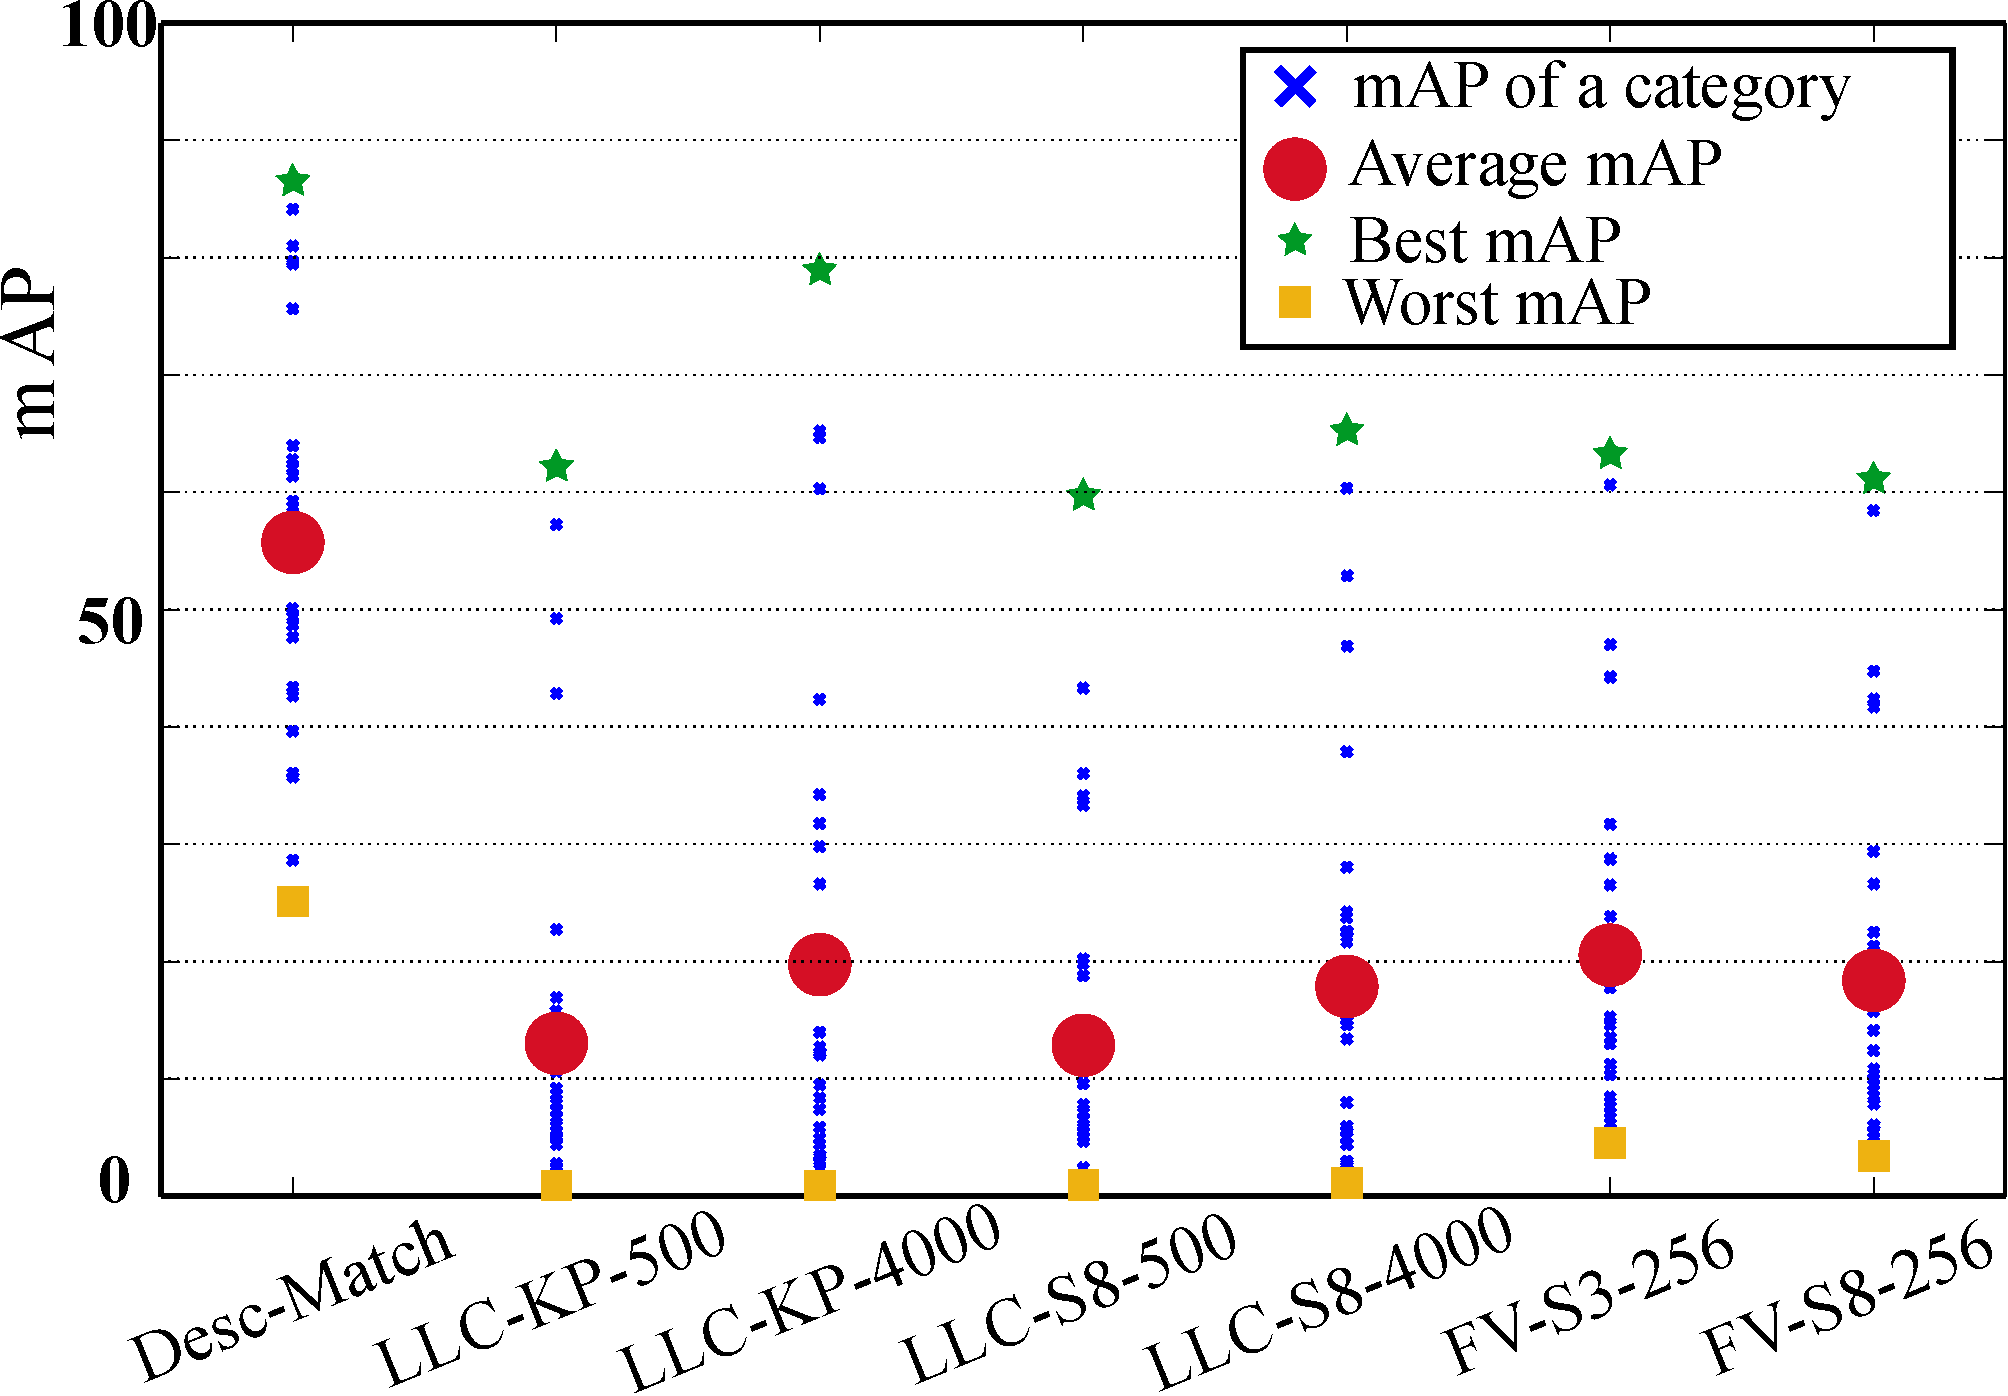
\includegraphics[width=\linewidth]{./gfx/Chapter03/methods-v5.pdf}
\caption{Detailed performance evaluation of state-of-the-art algorithms on SHORT. \textbf{LLC} -- locality-constrained linear coding; \textbf{FV} -- Fisher vector. The SIFT descriptors can be computed on dense grids with a spacing of \textbf{Sx} pixels or around the SIFT keypoints (\textbf{KP}). The last figure indicates the size of the visual vocabulary (256, 500 or 4000 visual words).}
\label{fig:methods}
\end{center}
\end{figure}



%% Old results

Classification results for the different methods are summarised in Table~\ref{table:classification_results}  and Fig.~\ref{fig:methods}. The low performance of most state-of-the-art methods demonstrates the challenge presented by SHORT. The precision/recall analysis shown in Fig.~\ref{fig:LLC-S8-4000} illustrates a remarkable variability in retrieval performance across categories. This fact reflects the complexity of the recognition problem, and the need for more robust algorithms. 

For example, recognition algorithms for hand-held objects should be able to either provide a good confidence measure, or possibly to request that further image queries be captured, even suggesting suitable, specific object transformations that could be used as a predictive verification step. For an assistive usage case, rather than a potentially incorrect match, it would be more appropriate for a system to reject the query.

\begin{figure}[h]
       \centering
		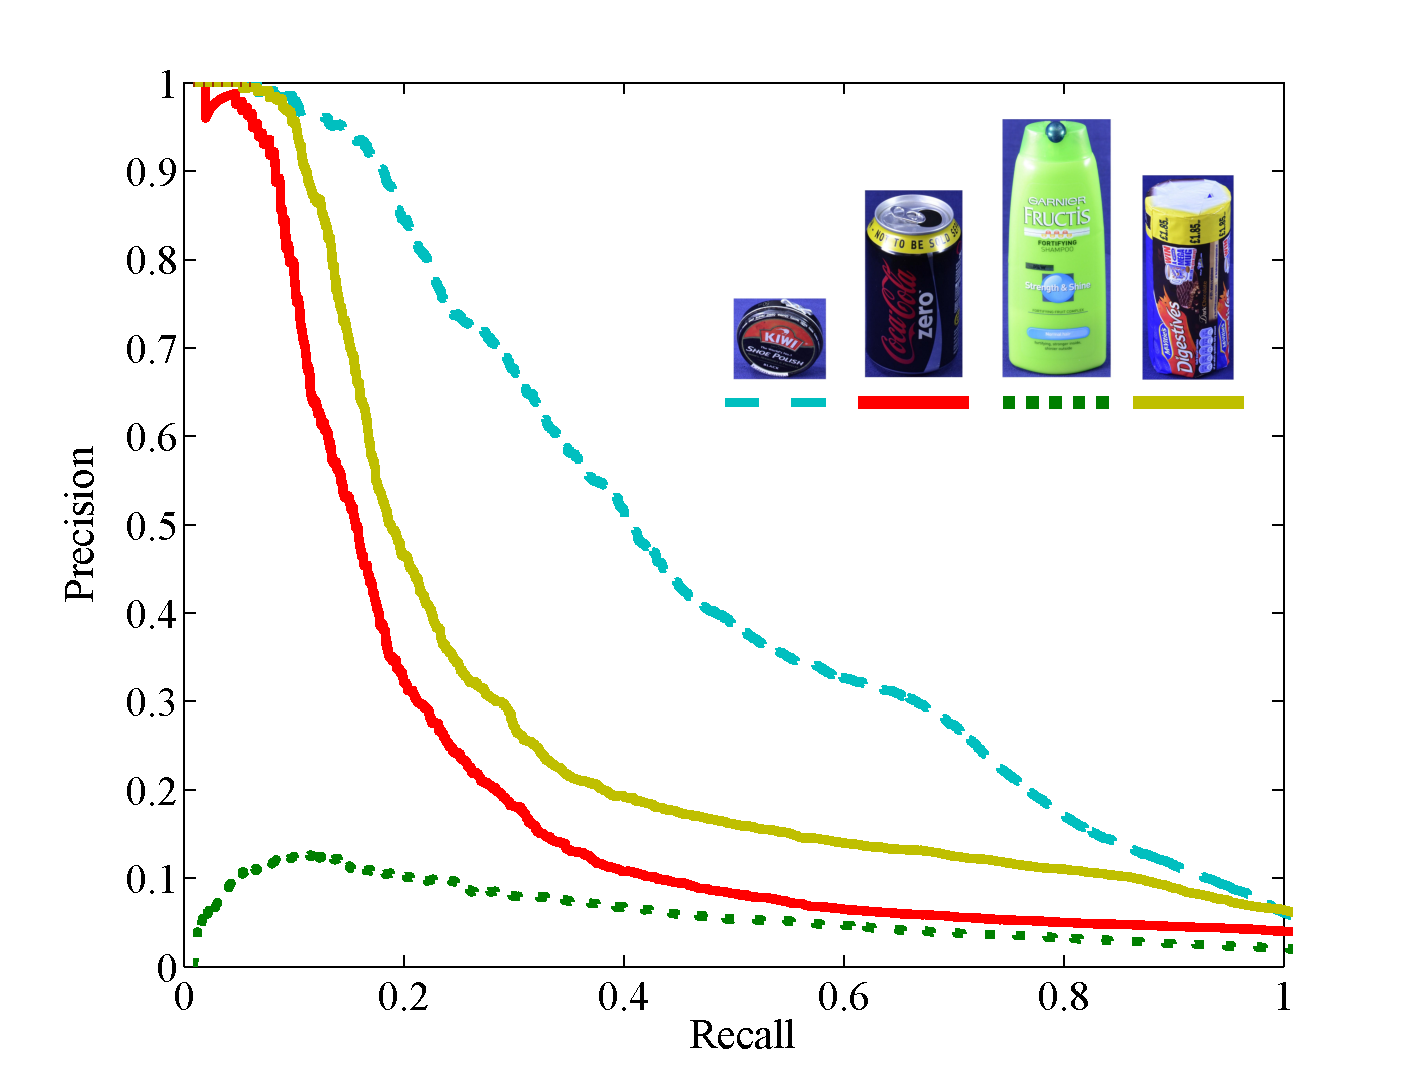
\includegraphics[width=\linewidth]{./gfx/Chapter03/precision-recall.pdf}
        \caption{LLC-S8-4000 Test. Representative empirical precision and recall curve for a small sample of product classes. Only four classes, including best and worst results, are represented to help visualisation. The test was run with 59,226 queries against the database of 1,080 models. Performance in all categories is summarised in Fig. \ref{fig:LLC-S8-4000}}
        \label{fig:LLC-S8-4000}
\end{figure}

Recently, the value of well-defined, robustly labelled datasets in both evaluating and training object recognition systems has become clear. Table~\ref{table:dataset_comparison}, provides a comparison of different datasets, and methods of recognition.  A few interesting observations may be made. For example, HA-4000 yields high average precision in the SHORT dataset, but appears to yield lower performance in Caltech-101 and PASCAL VOC databases. However, the results are the other way around for HA-500.  This suggests that a larger vocabulary is needed for the objects in SHORT. However, in the case of Caltech-101 where the images are of much lower resolution than SHORT, the details are not easily resolvable and hence a larger vocabulary captures irrelevant variations such as noise. Grozi-120 has a lower mAP than most of the SHORT groups, which is possibly due to its rather low spatial resolution. These observations suggest that we are still some way from having a single dataset that adequately represents all use cases for object recognition.


\begin{table}
\begin{center}
    \begin{tabular}{ccccc}
    \toprule
    mAP & VOC-2007 & Caltech-101 & SHORT-ST & SHORT-VF \\
	\midrule
    HA-4000                    & 37.50    & 18.91       & 45.86       & 36.86 \\
    HA-500                     & -        & 61.20       & 24.54       & 22.39       \\
    LLC-S8-4000                & 46.01    & 66.64       & 17.89       & 11.20       \\
    FV-S8-256                  & 59.35    & 77.78       & 18.39       & -           \\
	\bottomrule
    \end{tabular}
	\end{center}
    \caption{Dataset comparison. Classification results of baseline performance algorithms on SHORT and other existing datasets.}
    \label{table:dataset_comparison}
\end{table}


Furthermore, the categories in the dataset vary in shape, size, colour, etc. and therefore there is a large variability in classification accuracy across categories, which is reflected in Fig.~\ref{fig:LLC-S8-4000} and \ref{fig:ComplexMethodResults}. Products with low retrieval accuracy generally have reflective surfaces; the ones displaying high accuracy have clear surfaces with text labels, and are easy to hold and position. 



\begin{figure*}[t]
\centering
\subfloat[Dense sampling, CB = 4000 words.]{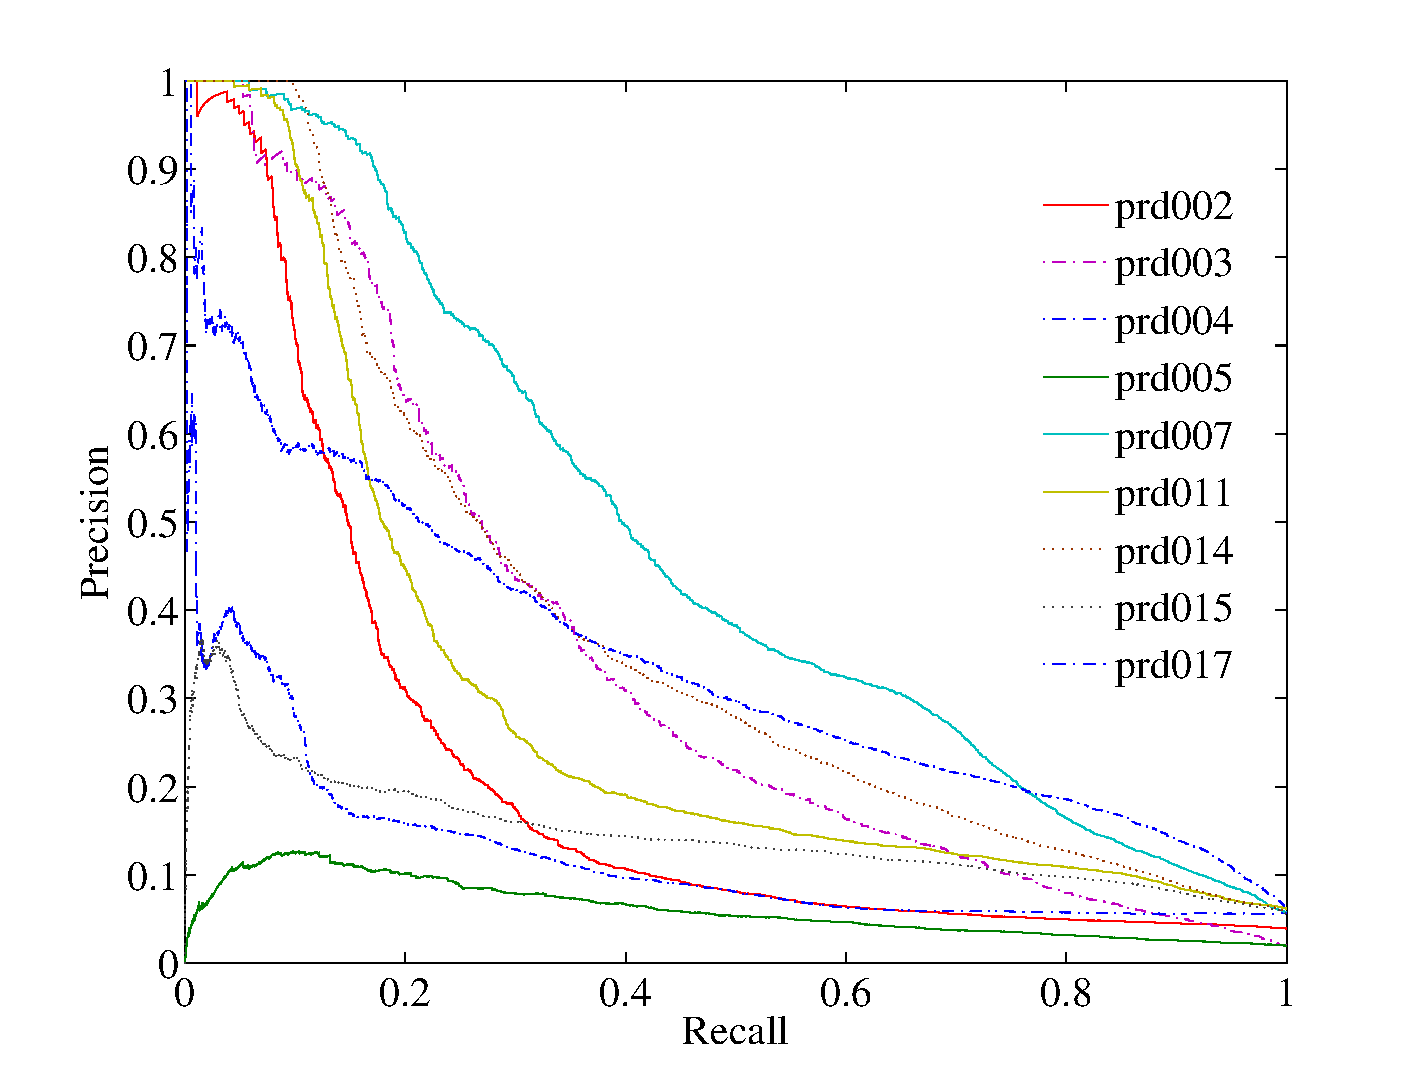
\includegraphics[width=.5\linewidth]{gfx/Chapter03/VFdense4000_new.pdf}}
\subfloat[Dense sampling, CB = 500 words.]{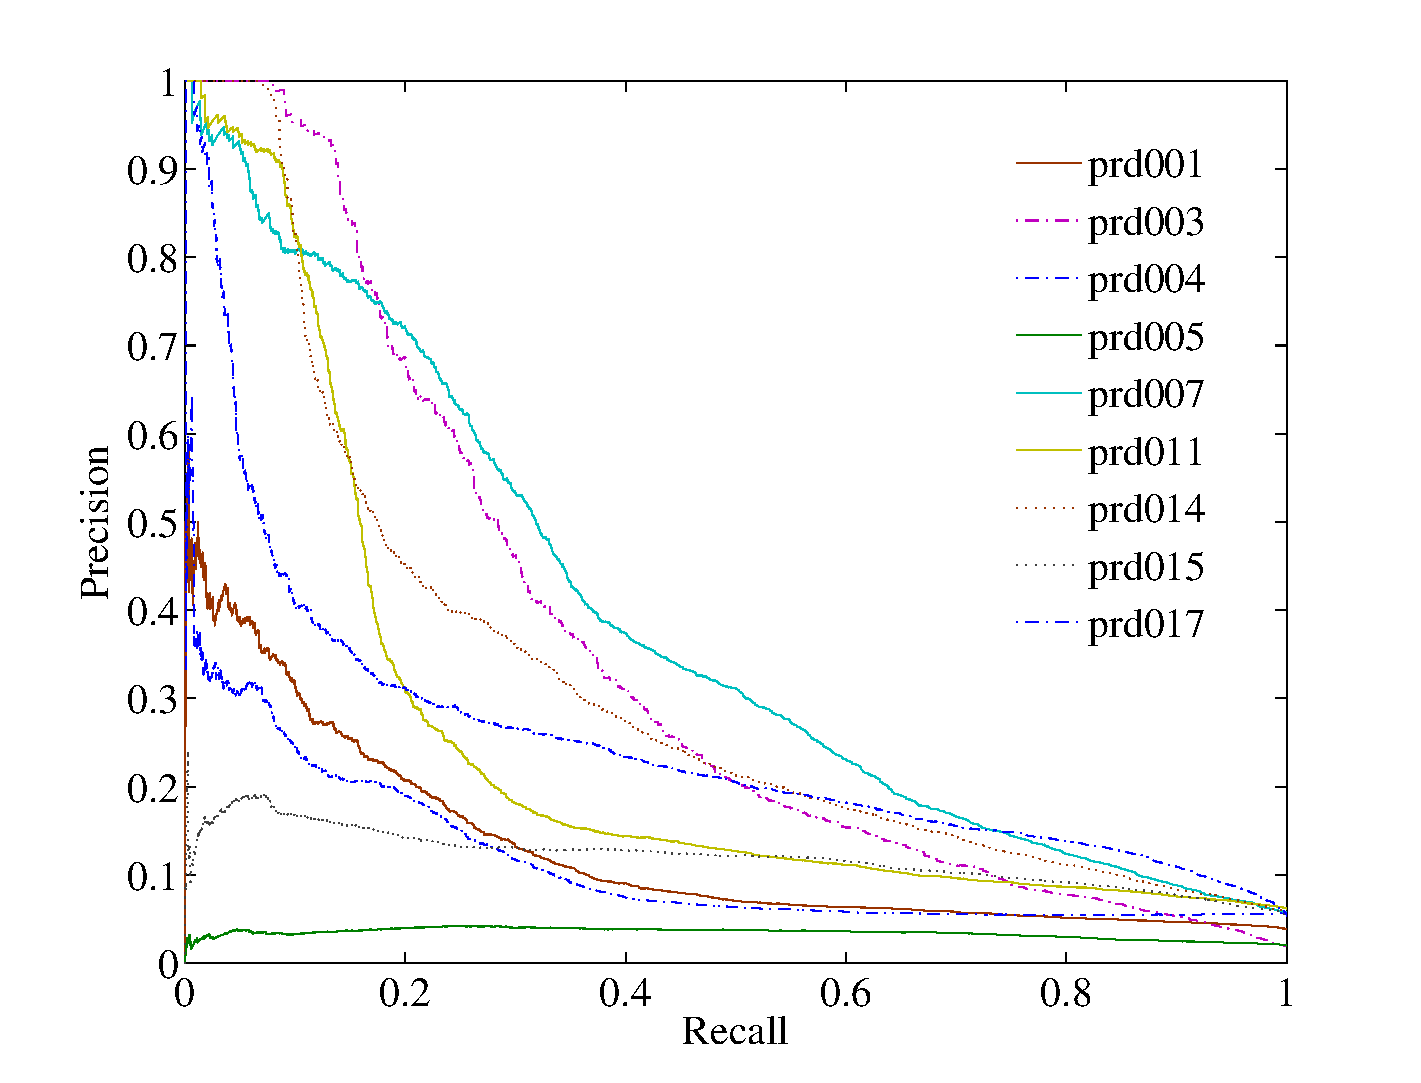
\includegraphics[width=.5\linewidth]{gfx/Chapter03/VFdense500_new.pdf}}


\subfloat[Sparse sampling, CB = 4000 words.]{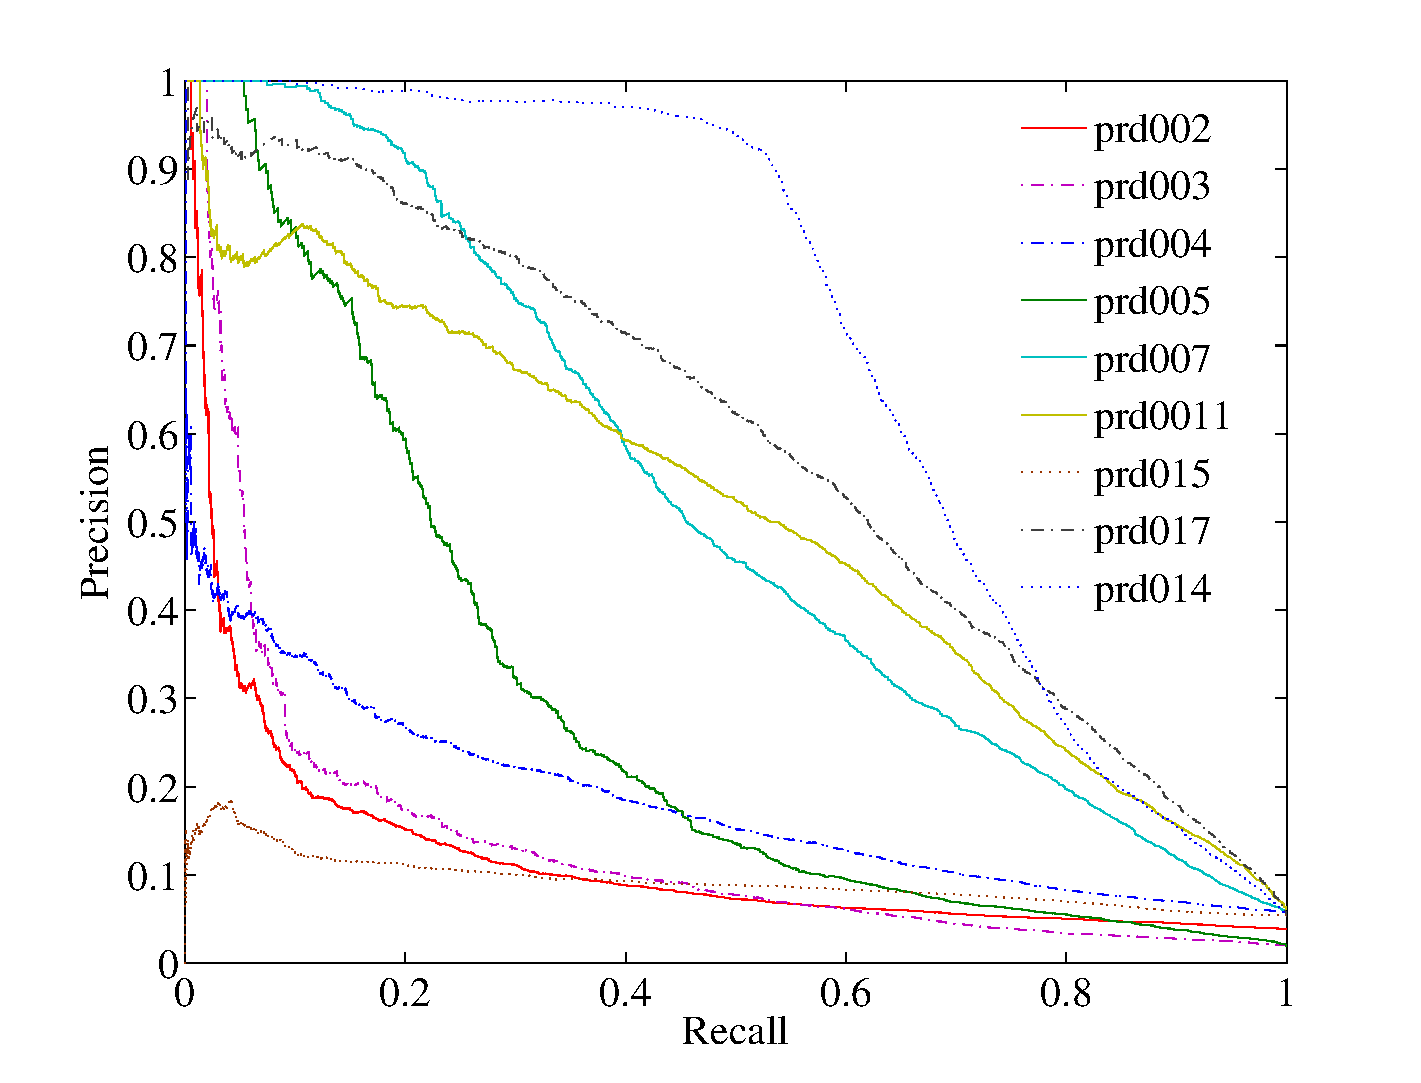
\includegraphics[width=.5\linewidth]{gfx/Chapter03/VFsparse4000_new.pdf}}
\subfloat[Sparse sampling, CB = 500 words.]{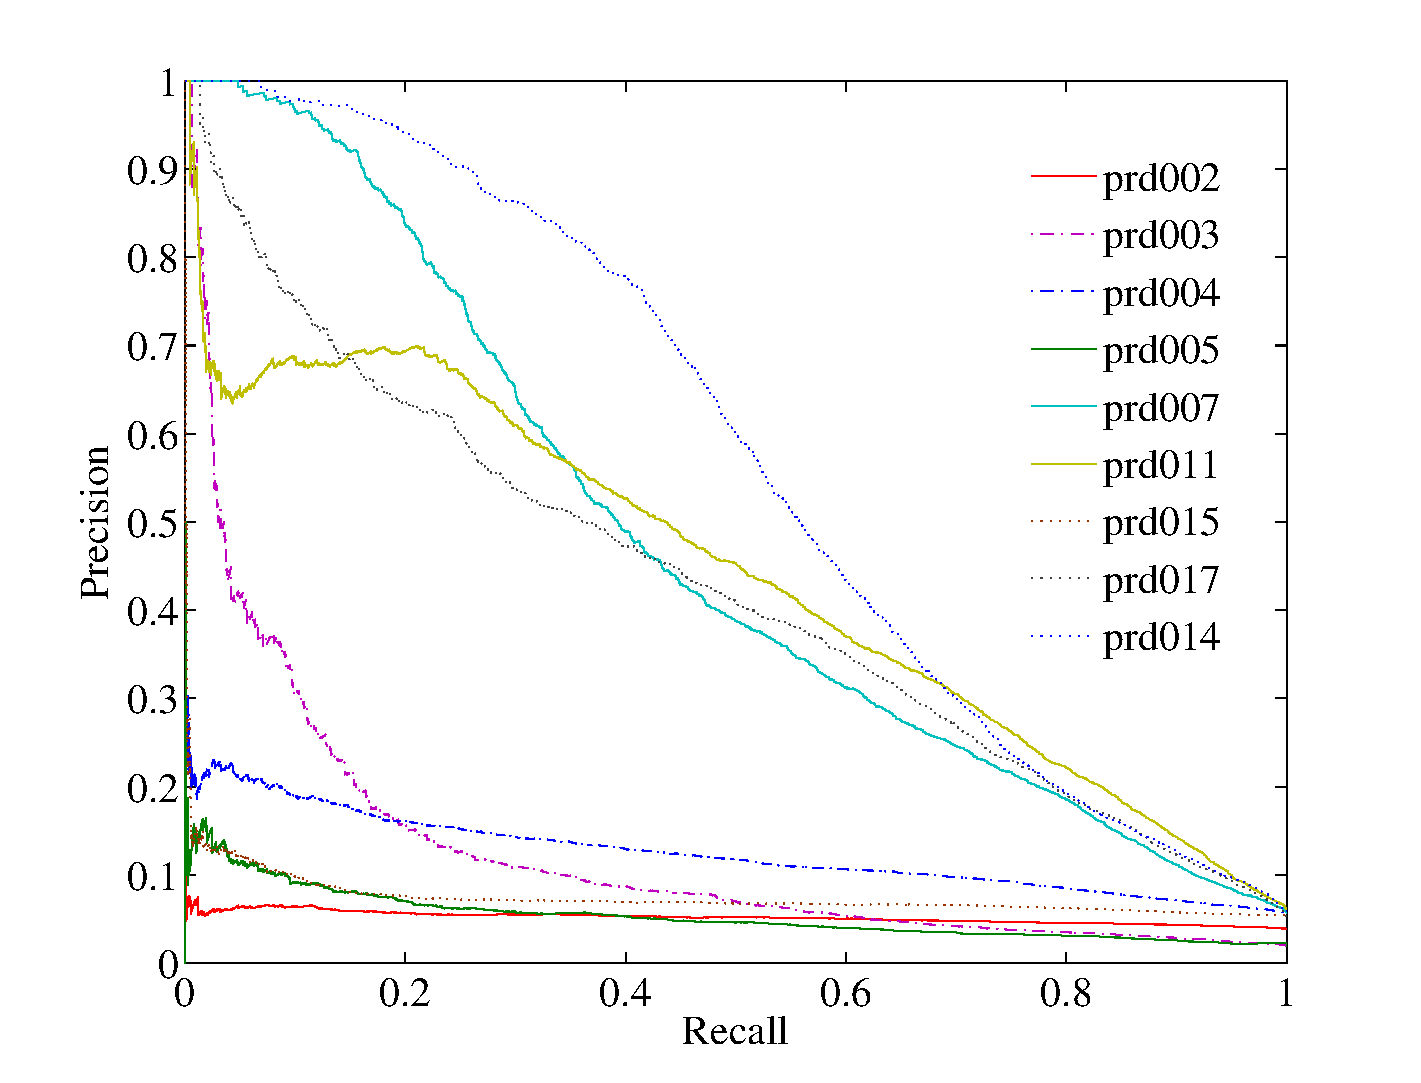
\includegraphics[width=.5\linewidth]{gfx/Chapter03/VFsparse500_new.pdf}}
\caption{BOVW + SVM test. Precision/recall curves for a representative sample of product classes: top four and worst five. The test was run with all the 59,226 queries against the database of 1,080 models.}
\label{fig:ComplexMethodResults}
\end{figure*}



% Figure on pose analysis


The range of training images in the database -- covering almost all faces of a product with three different elevations -- will enable further analysis regarding the training images required to ensure a minimum accuracy for recognition.  In this context, Figure~\ref{fig:poseAnalysisA} shows that increasing the training images do not necessarily improve the classification unless this increase conveys distinct information. The key factor is to include training images covering all faces of the product rather than different elevations. Figure~\ref{fig:poseAnalysisB} shows that most of the matches are made to the front view of an object since users tend to hold and identify products from this pose. Nevertheless, the scenario with blind and partially sighted users can be different, as images can be taken from any view.  Therefore, we have included a rich set of viewing angles in our training dataset so the computer vision community could benefit from this and increase the robustness of their methods in this particular context.



\begin{figure}[h]
\centering
\subfloat[]{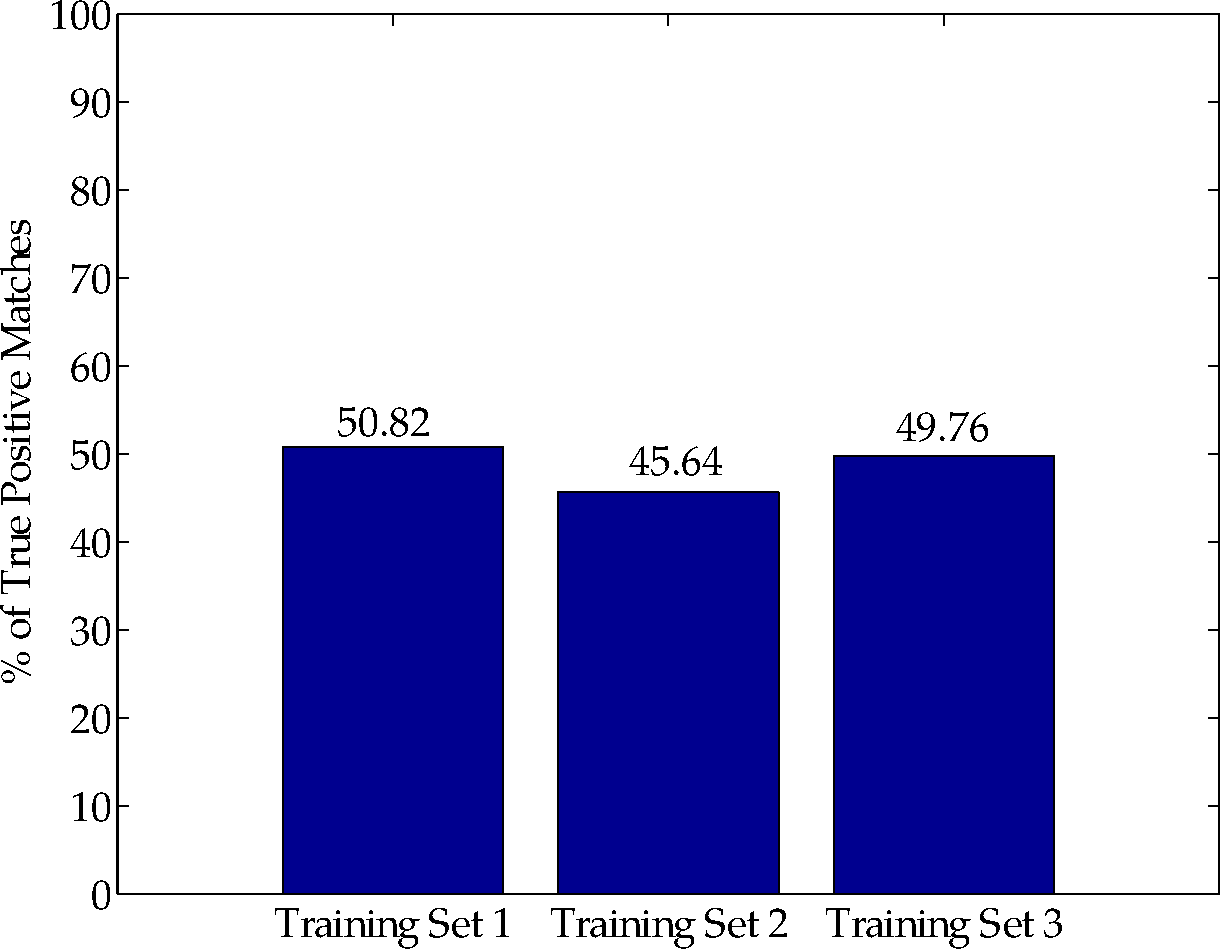
\includegraphics[width=\linewidth]{gfx/Chapter03/training-images-comparison-2.pdf}
\label{fig:poseAnalysisA}
}


\subfloat[]{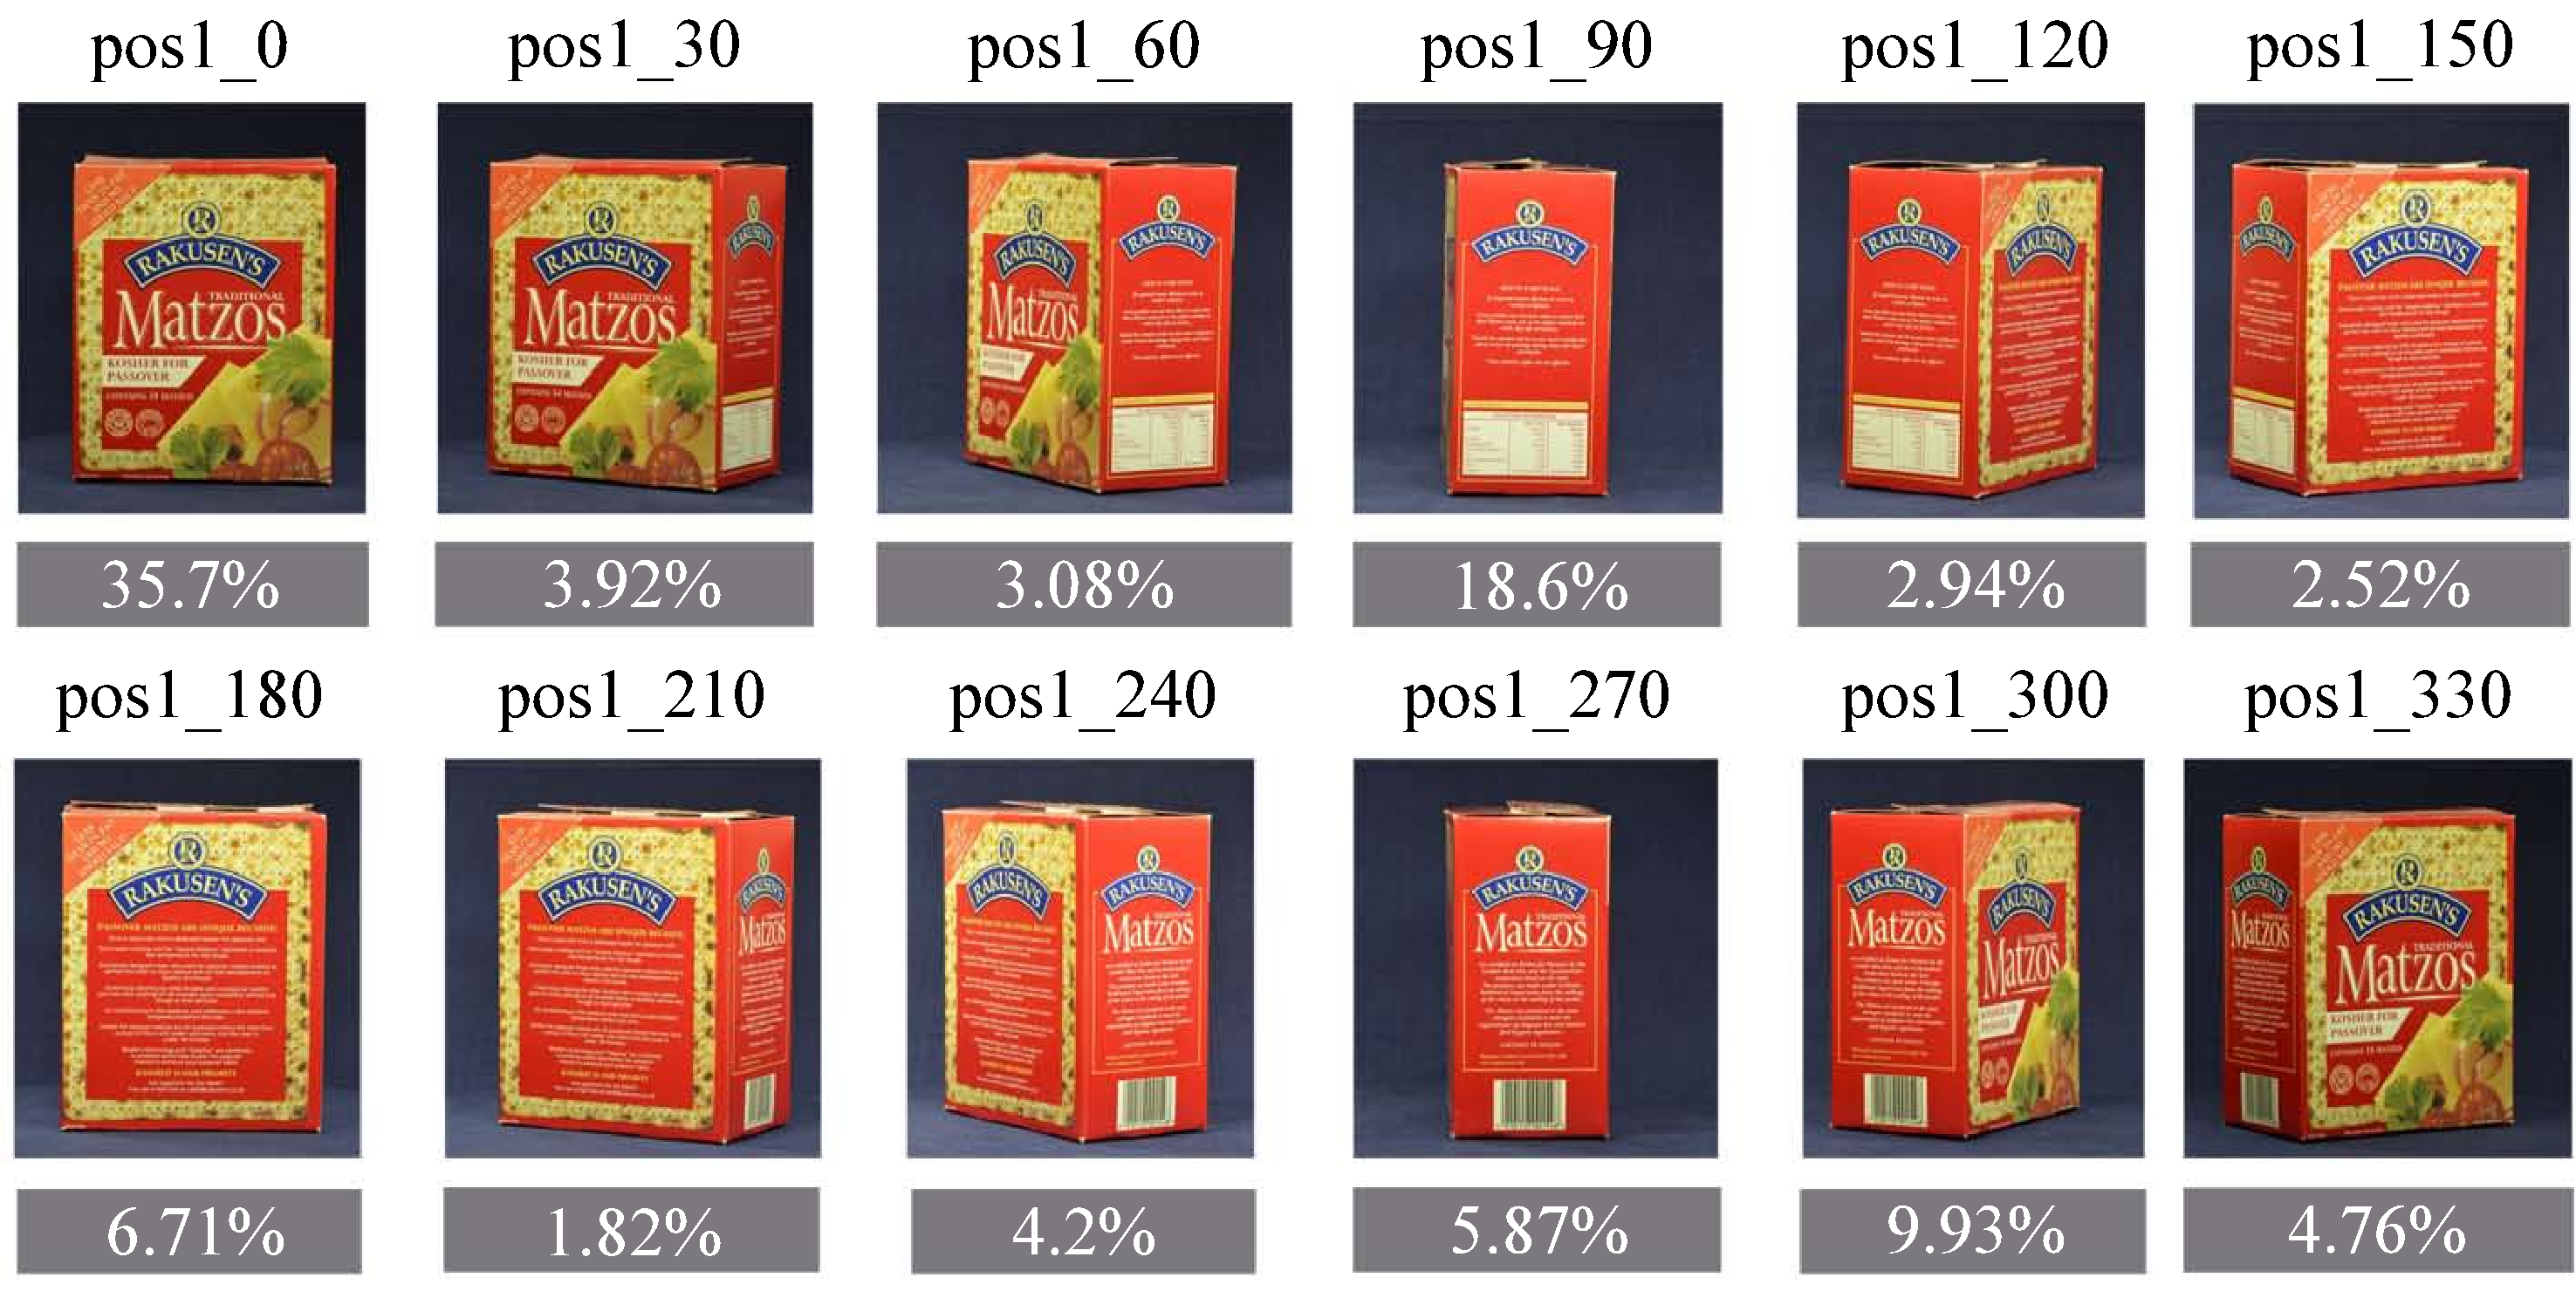
\includegraphics[width=\linewidth]{gfx/Chapter03/prd016_collage_72dpi.pdf}
\label{fig:poseAnalysisB}
}
\caption{SIFT descriptor matching. Analysis of the effect of using different training sets. Figure~\ref{fig:poseAnalysisA}: \textit{Training set 1} includes all the training images. \textit{Training set 2} contains 18 images of each product taken every $60^\circ$ at three different elevations. \textit{Training set 3} contains 12 images of each product at different angles but at the same elevation. A sample of \textit{Training set 3} with \textit{prd014: Matzos} is shown in Figure~\ref{fig:poseAnalysisB} with the \% of positive matches per position. This test was performed with 850 queries from the \textit{still-images} set.}
        \label{fig:poseAnalysis}
\end{figure}


\subsection{Evaluation of Sequential Video Frames} \label{subsec:evaluationframes}

In this section we analyse how we can use sequential frames from a video of an object in order to improve classification accuracy. First, multiple sequential images from a video were queried, and each image was matched to one of the thirty categories of the SHORT database using the descriptor matching as described in Sections~\ref{subsec:pairwise} and \ref{subsec:querydescrejection}. A histogram of the matches was computed for several videos of the same object, as shown in Fig.~\ref{fig:prd003a}. Even though the total number of incorrect matches increases as we query more video frames, they are distributed across a range of object categories in the database. 

\begin{figure}[htb]
\centering
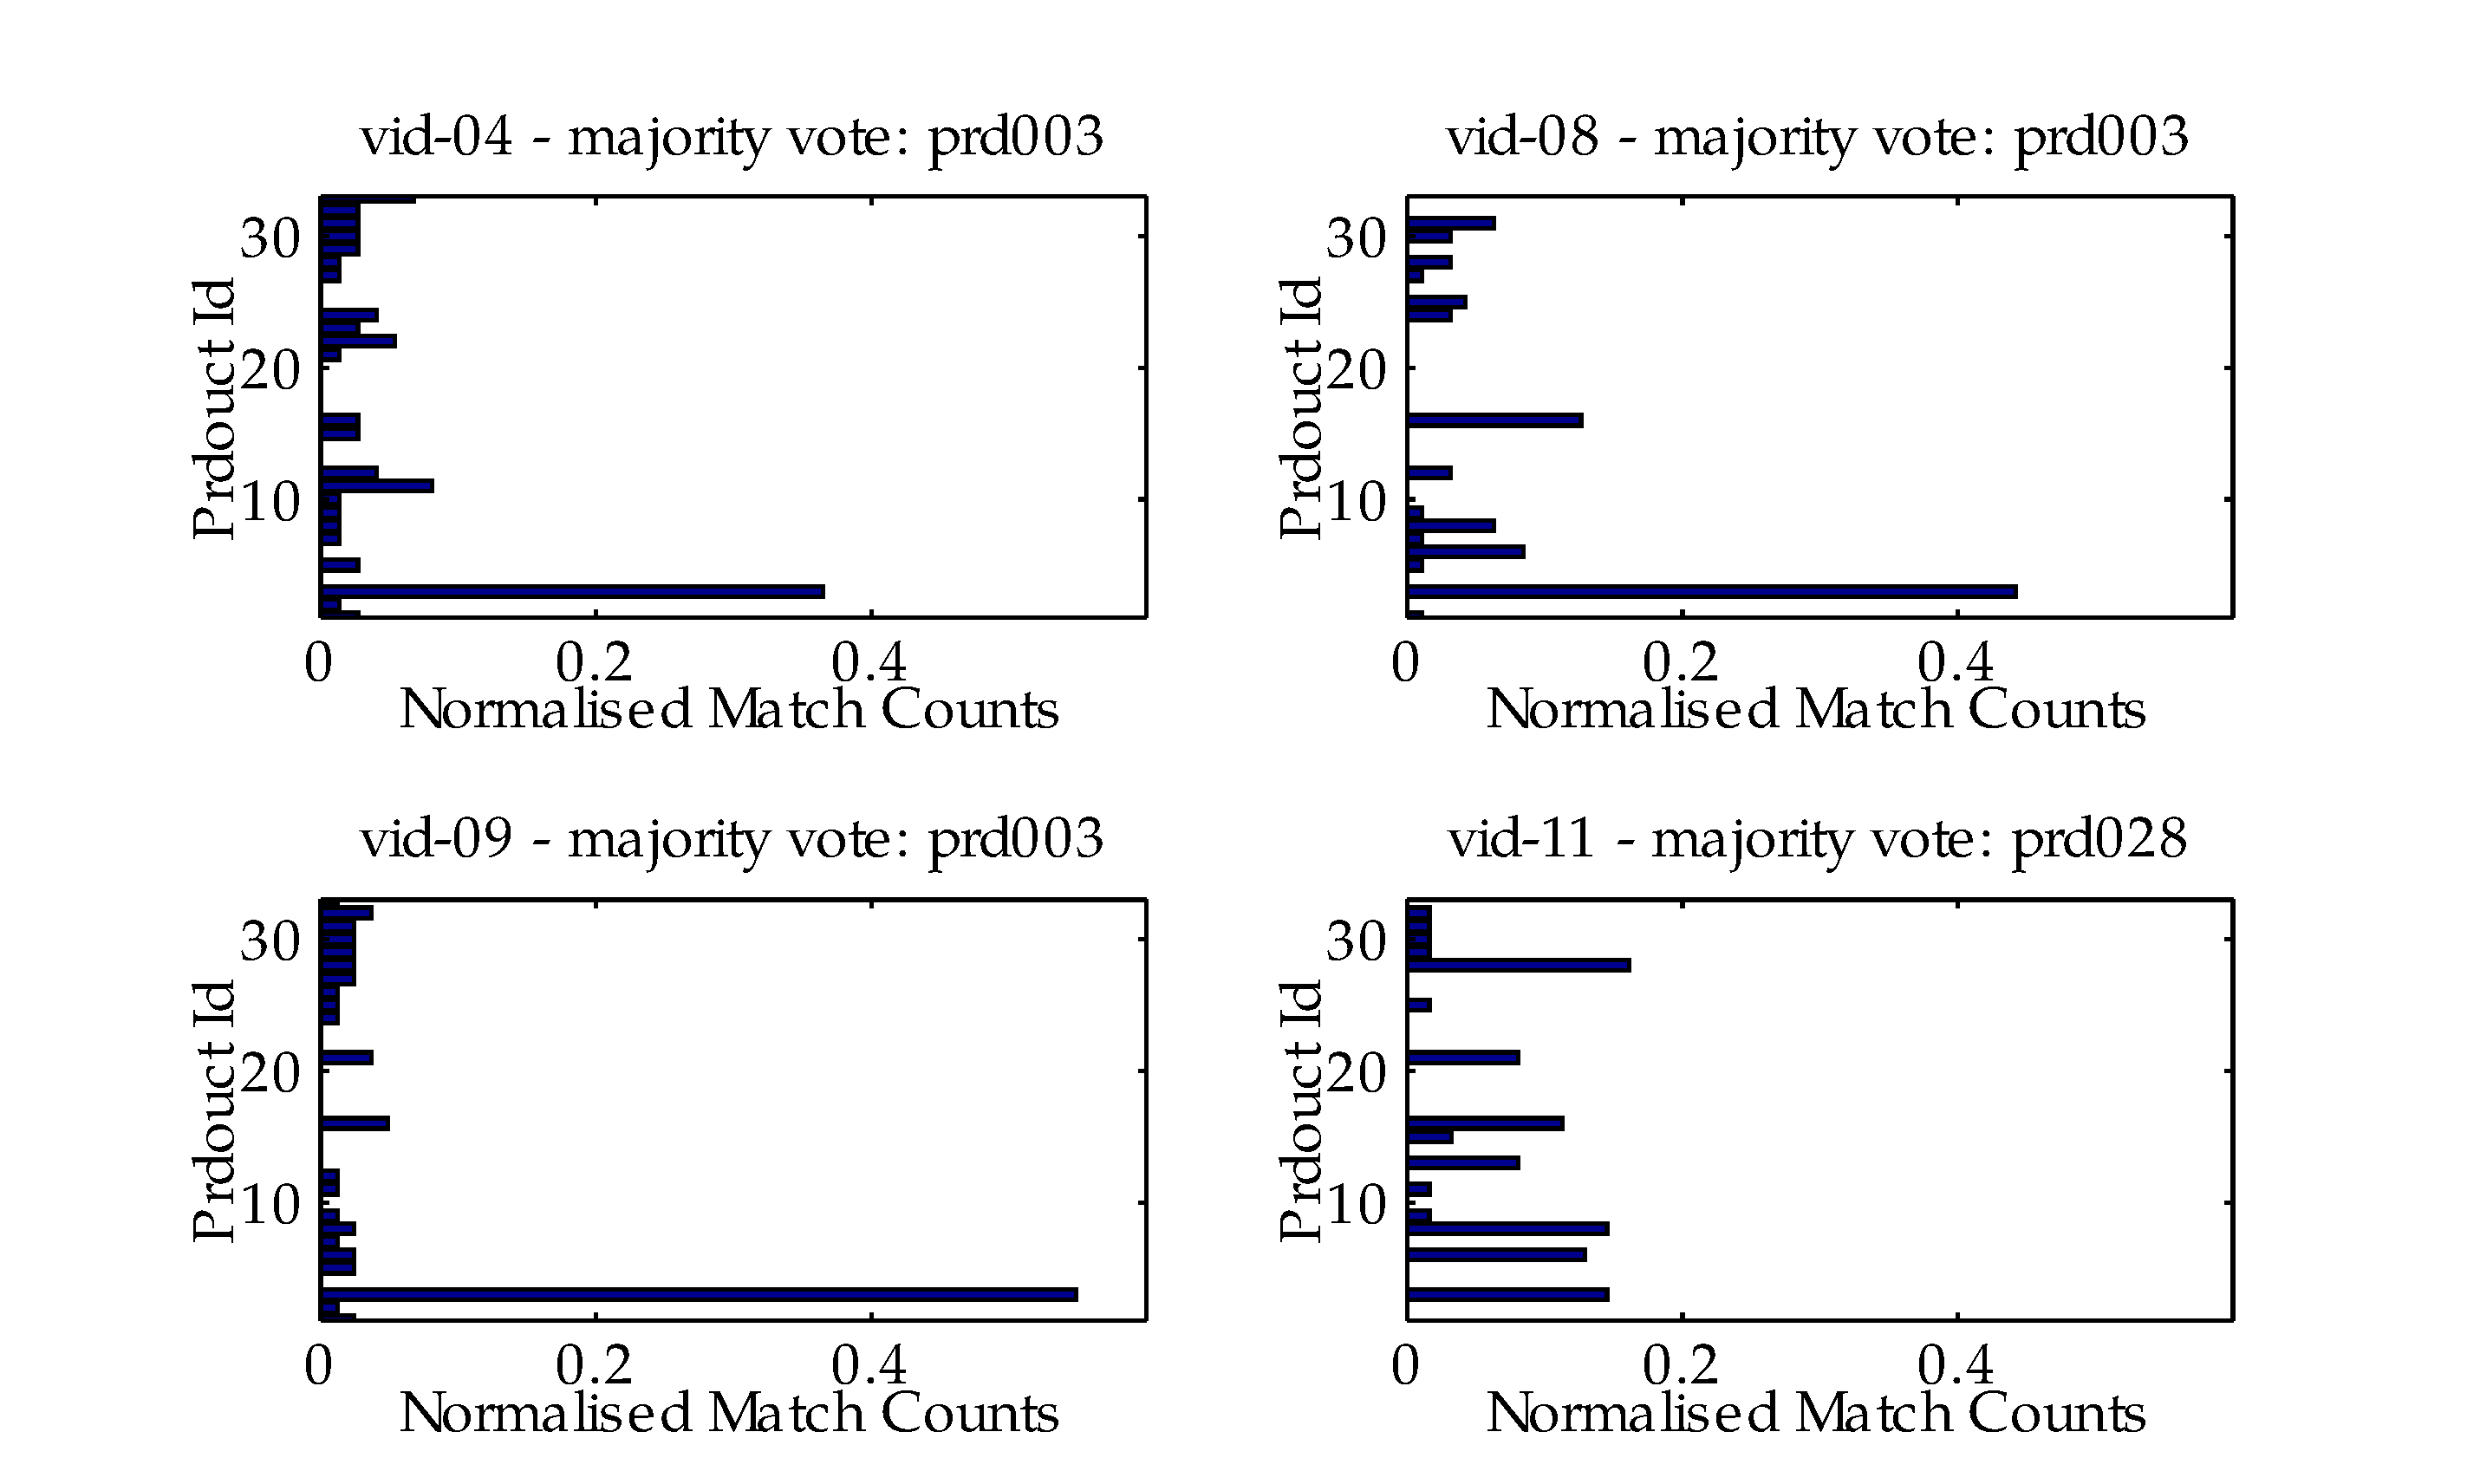
\includegraphics[width=\linewidth]{./gfx/Chapter02/prd003_distribution_bar-latex.pdf}
\caption{Evaluation of sequential video frames: Distribution of matches across different categories of SHORT dataset for four videos of the same query object.}
\label{fig:prd003a}
\end{figure}


As shown, the correct object often has a higher number of hits than the incorrect ones. Therefore we propose to use the ``individual voting'' as a metric to classify an object based on querying sequential images from a video of a hand-held object. Further analysis was undertaken in order to determine the number of video frames that are required for the total number of correct matches to exceed the number of individual total incorrect matches. Preliminary results, Figure \ref{fig:prd003b}, shows that the number of total incorrect matches to individual objects rises slowly while the number of total matches to the correct object increases rapidly. The above analyses were undertaken for several videos and object categories under the SHORT dataset. Classification accuracy using different numbers of query frames and the above metric is presented in Section~\ref{sec:expResults2}.


\begin{figure}[htb]
\centering
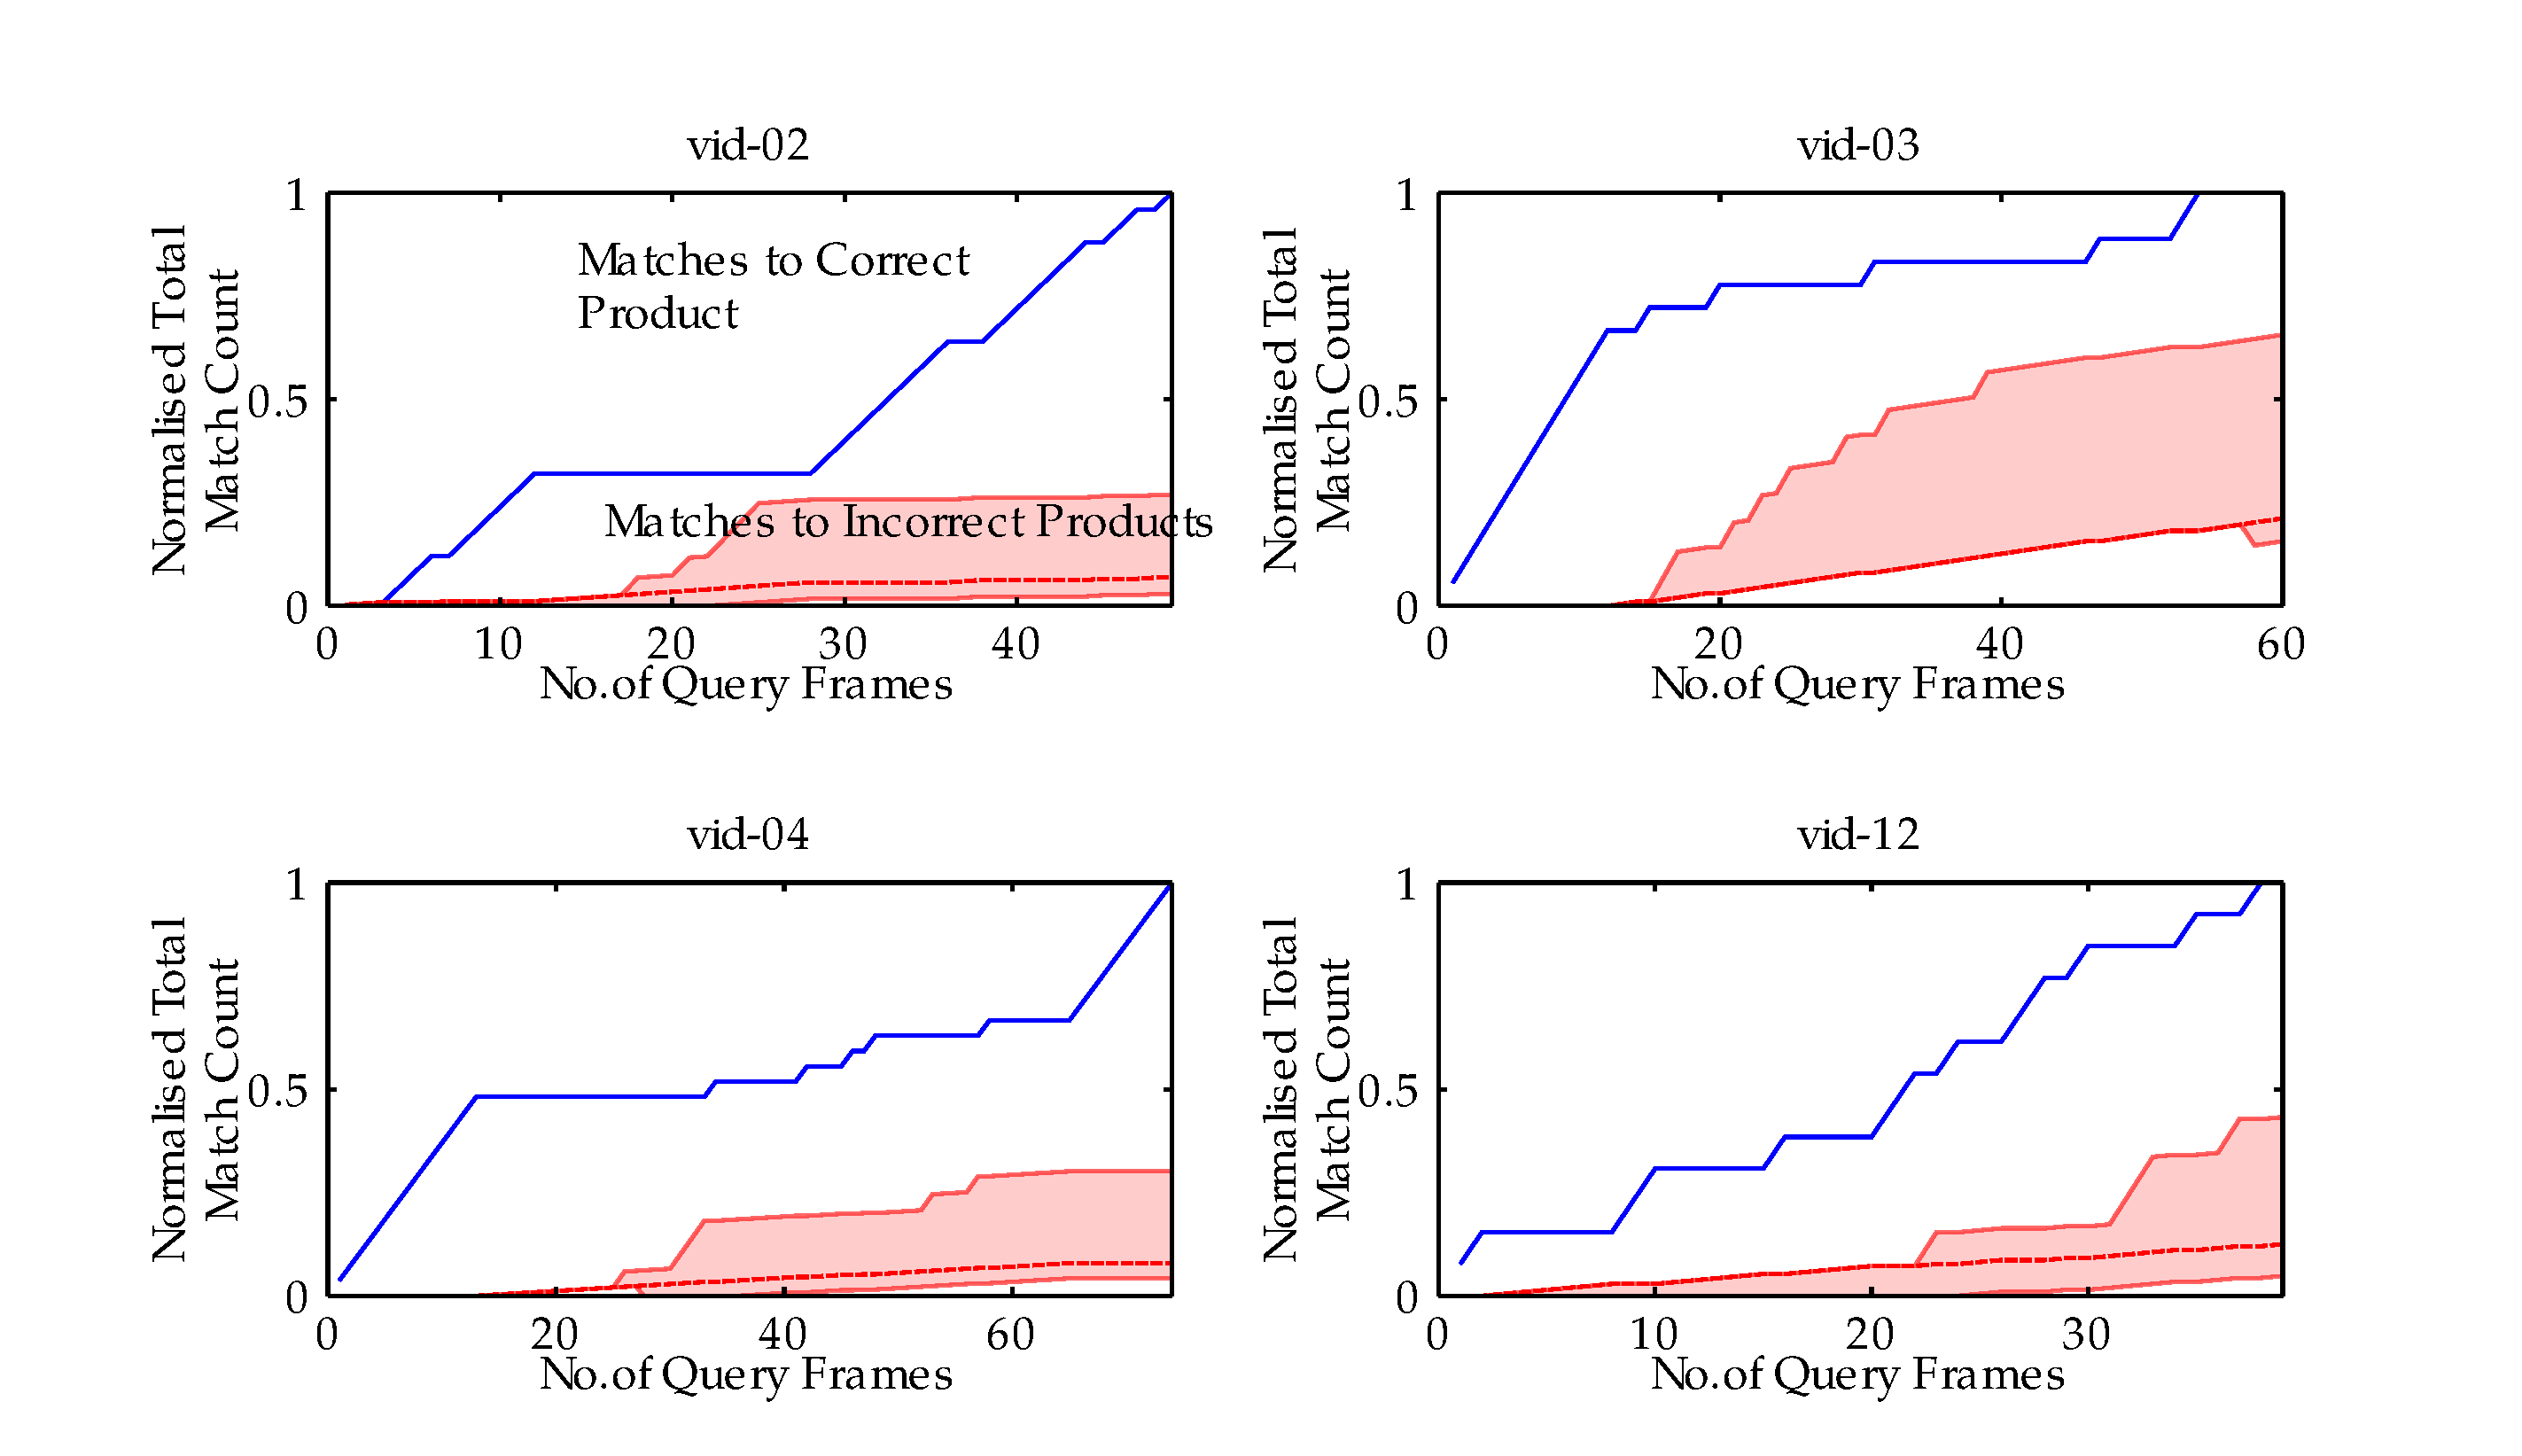
\includegraphics[width=\linewidth]{./gfx/Chapter02/prd0030shadedPlots-4-latex.pdf}
\caption{Evaluation of sequential video frames: Fraction of correctly matched queries to incorrect matches for videoframe sequences. Note that there is a distribution of incorrect matches across multiple categories as the number of sequential query frames increases.}        
\label{fig:prd003b}
\end{figure}


\subsection{Classification Accuracy Based on Sequential Video Frames} \label{sec:expResults2}

Classification accuracy using the individual voting metric (Section~\ref{subsec:evaluationframes}) was computed for six categories of SHORT dataset (Table~\ref{table:testData}). A video $\mathbf{Q}$, comprising of query frames $Q_i, i = 1,2,...,N$, is classified as the $k$-th category, $C_k$, to which the majority of query frames, $Q_i$, were matched to. The accuracy was calculated for classifying twelve videos of each object based on different limits for the number of queries allowed, $N$.

Table~\ref{table:testData} shows that the classification accuracy increases as we increase the limit of query frames, except for occasional dips which occur due to instability as a person rotates the object in their hand. In comparison to the classification accuracy of individual queries, classification based on sequential video frame queries gives a much higher accuracy.


\begin{table}
\centering
\begin{tabularx}{1.05\linewidth}{XXXXXXXXXXXX}
\toprule
& Single frame & \multicolumn{2}{c}{10 fr} & \multicolumn{2}{c}{30 fr} & \multicolumn{2}{c}{50 fr} & \multicolumn{2}{c}{70 fr} & \multicolumn{2}{c}{90 fr}\\
ID & Acc (\%) & Acc & Std & Acc & Std & Acc & Std & Acc & Std & Acc & Std \\
\midrule
1 & 37.9 & 85.7 & 35.0 & 85.7 & 35.0 & 85.7 & 35.0 & 92.9 & 25.8 & 92.9 & 25.8 \\
%\hline
2 & 55.6 & 75.0 & 43.3 & 75.0 & 43.3 & 66.7 & 47.1 & 75.0 & 43.3 & 91.7 & 27.6\\
%\hline
3 & 40.9 & 73.3 & 44.2 & 73.3 & 44.2 & 80.0 & 40.0 & 80.0 & 40.0 & 80.0 & 40.0\\
%\hline
5 & 43.1 & 62.5 & 48.4 & 62.5 & 48.4 & 62.5 & 48.4 & 87.5 & 33.1  & 87.5 & 33.1\\
%\hline
6 & 80.6 & 92.3 & 26.7 & 100.0 & 0.0 & 100.0 & 0.0 & 100.0 & 0.0  & 100.0 & 0.0\\
%\hline
7 & 46.2 & 78.6 & 41.0 & 78.6 & 41.0 & 92.9 & 25.8 & 92.9 & 25.8  & 92.9 & 25.8\\
\bottomrule
\end{tabularx}
\caption{Classification accuracy of different objects for different number of sequential query frames (fr). Accuracy is defined as the number of videos correctly classified divided by the total number of videos queried.}
\label{table:testData}
\end{table}





%\begin{table}
%\centering
%\begin{tabularx}{1.2\linewidth}{XXXXXXXXXXXX}
%\toprule
% ID& Single frame & \multicolumn{2}{c}{10 frames} & \multicolumn{2}{c}{30 frames} & \multicolumn{2}{c}{50 frames} & \multicolumn{2}{c}{70 frames} & \multicolumn{2}{c}{90 frames}\\
% & Acc (\%) & Acc & Std & Acc & Std & Acc & Std & Acc & Std & Acc & Std \\
%\midrule
%1 & 37.89 & 85.71 & 34.99 & 85.71 & 34.99 & 85.71 & 34.99 & 92.86 & 25.75 & 92.86 & 25.75 \\
%%\hline
%2 & 55.56 & 75.00 & 43.30 & 75.00 & 43.30 & 66.67 & 47.14 & 75.00 & 43.30 & 91.67 & 27.64\\
%%\hline
%3 & 40.87 & 73.33 & 44.22 & 73.33 & 44.22 & 80.00 & 40.00 & 80.00 & 40.00 & 80.00 & 40.00\\
%%\hline
%5 & 43.14 & 62.50 & 48.41 & 62.50 & 48.41 & 62.50 & 48.41 & 87.50 & 33.07  & 87.50 & 33.07\\
%%\hline
%6 & 80.61 & 92.31 & 26.65 & 100.00 & 0.00 & 100.00 & 0.00 & 100.00 & 0.00  & 100.00 & 0.00\\
%%\hline
%7 & 46.15 & 78.57 & 41.03 & 78.57 & 41.03 & 92.86 & 25.75 & 92.86 & 25.75  & 92.86 & 25.75\\
%\bottomrule
%\end{tabularx}
%\caption{Classification accuracy of different objects for different number of sequential query frames. Accuracy is defined as the number of videos correctly classified divided by the total number of videos queried.}
%\label{table:testData}
%\end{table}



%%------------------------------------------------------------------------
\section{Conclusion and Future Work} \label{sec:conclusions}

We have presented a new publicly available  dataset containing queries consisting of single images and video frames of hand-held objects.  These were captured by multiple users using a variety of smartphones. The purpose of this dataset set is to have a more realistic view of variability in acquisition across images taken of hand-held objects. Unlike other datasets, SHORT also contains a great disparity in the image resolution and quality of its object and query items, which we feel is more representative of conditions of use we would expect for high-quality, curated models being used to service queries from wearable of hand-held cameras.

The training set of model images systematically captures variations in objects' viewing angle allowing us to study the effect of the number of viewing angles present in a database on matching quality in a widely varying query. SHORT can be used to develop object recognition algorithms targeted for both sighted and visually-impaired users: comparisons of such will allow a better understanding of the extra technical requirements placed on computer vision systems by users who may not be aware of the quality of the images they are capturing. Additionally, SHORT paves the way for addressing several open questions; for example:

\begin{enumerate}[a)]
\item How to minimise -- or better yet, eliminate -- the chance of a false positive match. Such errors could be dangerous when used in the context of household product identification. SHORT, with a range of variability in the test images, can be used to establish image quality metrics for accepting a query in this context.

\item How to ensure that ambiguity between two similar products might be noted and used to either eliminate a candidate search result as being too uncertain a match, or to prompt a user to submit specific queries based around competing hypotheses of what the object might be.
\end{enumerate}



A key issue is that of how to minimise -- or better yet, eliminate -- the chance of a false positive match: such errors could be dangerous when used in the context of household product identification. One way to tackle this would be to reject a query based partly on its quality (sharpness, resolution, etc.). SHORT, with a range of variability in the test images, can be used to establish image quality metrics for accepting a query in this context. Another possibility would be to reject a query based on the degree of visual ambiguity, when assessed against the database. This brings us to the question of database size.

Scalability of image search in large databases brings a key challenge: how to ensure that ambiguity between two similar products might be noted and used to either eliminate a candidate search result as being too uncertain a match, or to prompt a user to submit specific queries based around different hypotheses of what the object might be. 

SHORT was developed with the intention of piloting a larger dataset to test such strategies, and indeed our future work will aim to increase the number of classes. We are currently exploring curated crowdsourcing techniques to involve a larger community in growth of the dataset.

Our first step towards this goal is to involve the potential dataset users in its expansion and we are studying how to convert the download website \url{http://short.bicv.org} into a portal for crowdsourcing of grocery pictures and the benchmark of third party algorithms against the SHORT dataset.

The shopping and assistive contexts pose a real challenge for the current generation of recognition algorithms, and SHORT represents a key step towards being able to assess performance under realistic query conditions.




%*****************************************
%*****************************************
%*****************************************
%*****************************************
%*****************************************
